\documentclass[a4paper]{beamer}%handout


\usepackage{listings}
\usepackage{color}
 
\definecolor{codegreen}{rgb}{0,0.6,0}
\definecolor{codegray}{rgb}{0.5,0.5,0.5}
\definecolor{codepurple}{rgb}{0.58,0,0.82}
\definecolor{backcolour}{rgb}{0.95,0.95,0.92}


%% Add Matlab code
\usepackage{mcode}
%% Add Matlab code end


%% Add watermarks
%\usepackage{draftwatermark}
%% Add watermarks end
\usepackage[utf8]{inputenc}
\usepackage{multicol}
\usepackage{url}
\usepackage{hyperref}
\hypersetup{
	colorlinks=true,
	linkcolor=cyan,          % color of internal links (change box color with linkbordercolor)
    citecolor=green,        % color of links to bibliography
    filecolor=magenta,      % color of file links
    urlcolor=cyan           % color of external links
	}

\graphicspath{{img/}}

\mode<presentation> {

%\usetheme{default}%yes % use %\frametitle in all slides recommended
%\usetheme{AnnArbor}%no
%\usetheme{Antibes} %yes %favorite
%\usetheme{Bergen} %no
%\usetheme{Berkeley} %no
%\usetheme{Berlin} %no
%\usetheme{Boadilla} %yes % good use of paper space
%\usetheme{CambridgeUS} %yes %favorite %use %\frametitle recommended
%\usetheme{Copenhagen}%yes%noframetitle
%\usetheme{Darmstadt}%no
%\usetheme{Dresden}
%\usetheme{Frankfurt}
%\usetheme{Goettingen}
%\usetheme{Hannover}
%\usetheme{Ilmenau}%no
%\usetheme{JuanLesPins}
%\usetheme{Luebeck}
%\usetheme{Madrid}
%\usetheme{Malmoe}
%\usetheme{Marburg}
%\usetheme{Montpellier}
%\usetheme{PaloAlto}
%\usetheme{Pittsburgh}%no
%\usetheme{Rochester}%no
%\usetheme{Singapore}%yees
%\usetheme{Szeged}%no
%\usetheme{Warsaw}%no

% As well as themes, the Beamer class has a number of color themes
% for any slide theme. Uncomment each of these in turn to see how it
% changes the colors of your current slide theme.

%\usecolortheme{albatross}
%\usecolortheme{beaver}
%\usecolortheme{beetle}
%\usecolortheme{crane}
\usecolortheme{dolphin}
%\usecolortheme{dove}
%\usecolortheme{fly}
%\usecolortheme{lily}
%\usecolortheme{orchid}
%\usecolortheme{rose}
%\usecolortheme{seagull}
%\usecolortheme{seahorse}
%\usecolortheme{whale}
%\usecolortheme{wolverine}

\setbeamertemplate{footline} % To remove the footer line in all slides uncomment this line
%\setbeamertemplate{footline}[page number] % To replace the footer line in all slides with a simple slide count uncomment this line

\setbeamertemplate{navigation symbols}{} % To remove the navigation symbols from the bottom of all slides uncomment this line
}

%----------------------------------------------------------------------------------------
%	NEW COMMANDS
%----------------------------------------------------------------------------------------

\newcommand{\Conv}{\mathop{\scalebox{1.5}{\raisebox{-0.2ex}{$\ast$}}}}%
%\linespread{1.3}

%----------------------------------------------------------------------------------------
%	TITLE PAGE
%----------------------------------------------------------------------------------------

\title[Introduction]{Digital Image Processing} % The short title appears at the bottom of every slide, the full title is only on the title page

\author{Prof. Tiago Vieira} % Your name
\institute[UFAL] % Your institution as it will appear on the bottom of every slide, may be shorthand to save space
{
Universidade Federal de Alagoas \\ % Your institution for the title page
\medskip
\textit{tvieira@ic.ufal.br} % Your email address
}
\date{\today} % Date, can be changed to a custom date


%----------------------------------------------------------------------------------------
%	TITLE PAGE
%----------------------------------------------------------------------------------------

\title[Segmentation]{Image Formation} % The short title appears at the bottom of every slide, the full title is only on the title page

\author{Prof. Tiago Vieira} % Your name
\institute[UFAL] % Your institution as it will appear on the bottom of every slide, may be shorthand to save space
{
Universidade Federal de Alagoas \\ % Your institution for the title page
\medskip
\textit{tvieira@ic.ufal.br} % Your email address
}
\date{\today} % Date, can be changed to a custom date

%------------------------------------------------

\begin{document}

%------------------------------------------------

\begin{frame}
\titlepage % Print the title page as the first slide
\end{frame}

\begin{frame}{Contents}
\setcounter{tocdepth}{1}
\tableofcontents
\end{frame}

%------------------------------------------------

\section{Introduction}

\begin{frame}
\centering
\begin{figure}[!h]
\centering
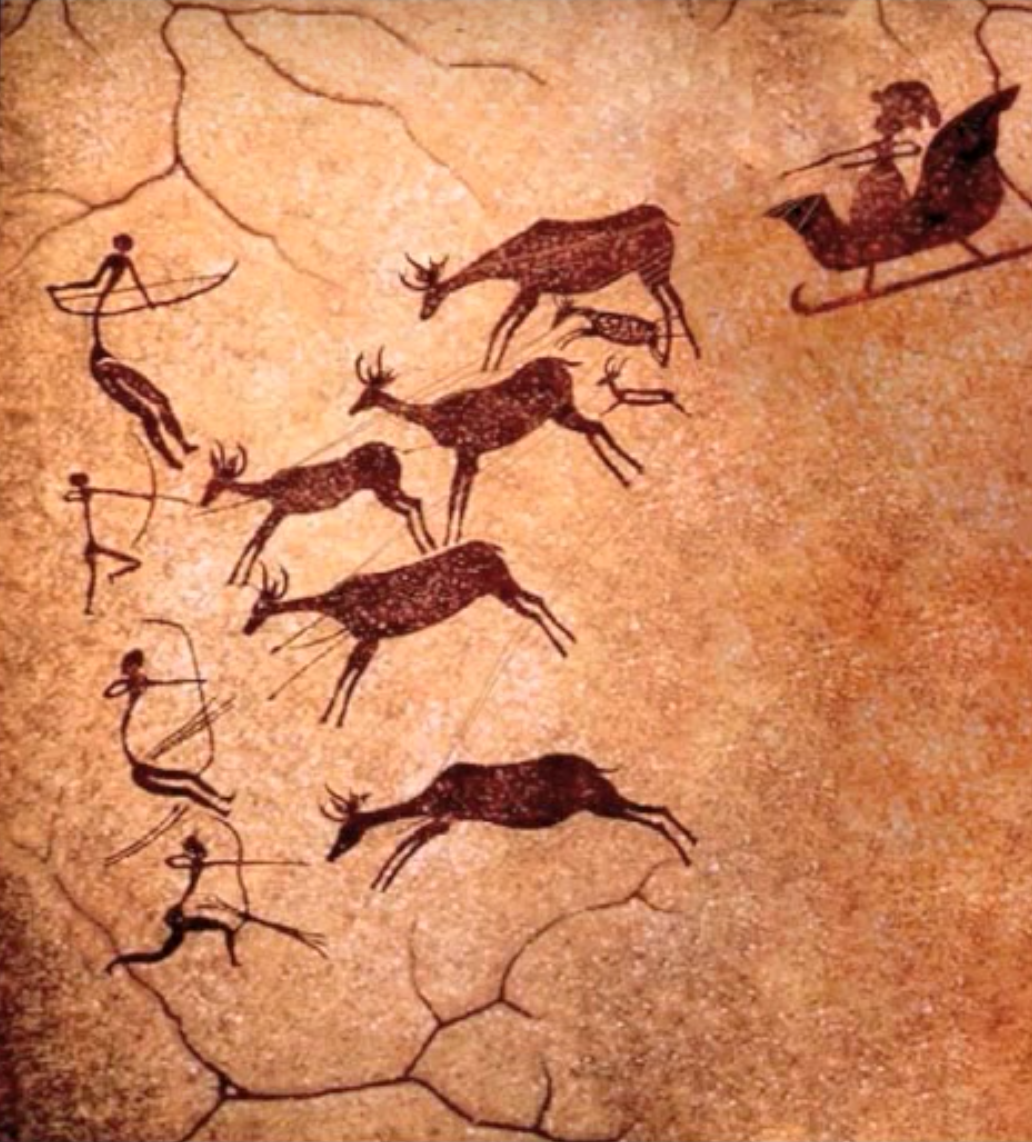
\includegraphics[width=.5\textwidth]{cave}
\end{figure}
Cave paintings $\approx$40.000 years ago
\end{frame}

\begin{frame}
\begin{block}{Forced perspective}
is a technique which employs optical illusion to make an object appear farther away, closer, larger or smaller than it actually is. It manipulates human visual perception through the use of scaled objects and the correlation between them and the vantage point of the spectator or camera. It has applications in photography, filmmaking and architecture.
\end{block}
\end{frame}

\begin{frame}
\centering
\begin{figure}[!h]
\centering
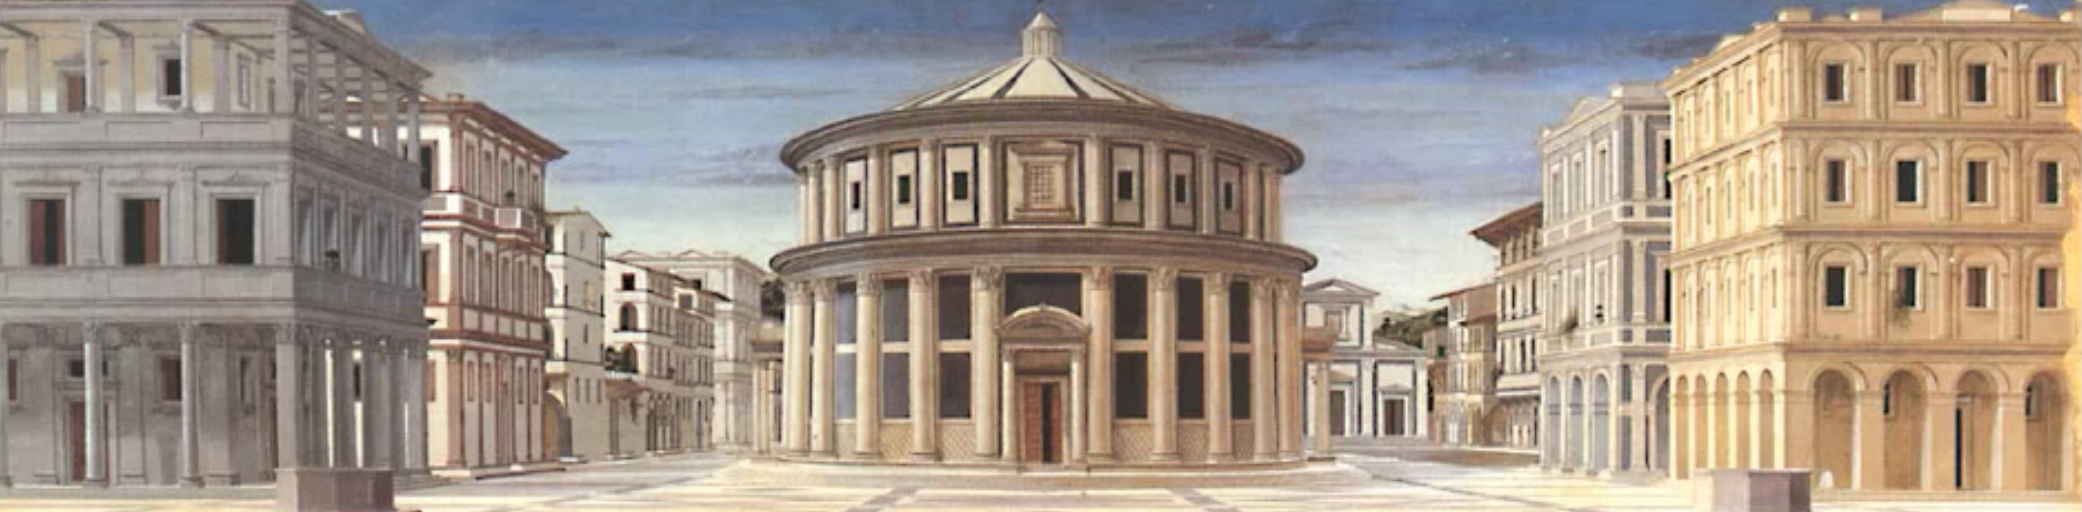
\includegraphics[width=\textwidth]{pietro}
\end{figure}
Pietro della Francesca (1415-1492)
\end{frame}

\begin{frame}
\begin{columns}
\begin{column}{.5\textwidth}
\begin{block}{\textit{Trompe-l'œil} (French for ``deceive the eye'')}
{is an art technique that uses realistic imagery to create the optical illusion that the depicted objects exist in three dimensions. Forced perspective is a comparable illusion in architecture.}
\end{block}
\end{column}
\begin{column}{.5\textwidth}
\begin{figure}[!h]
\centering
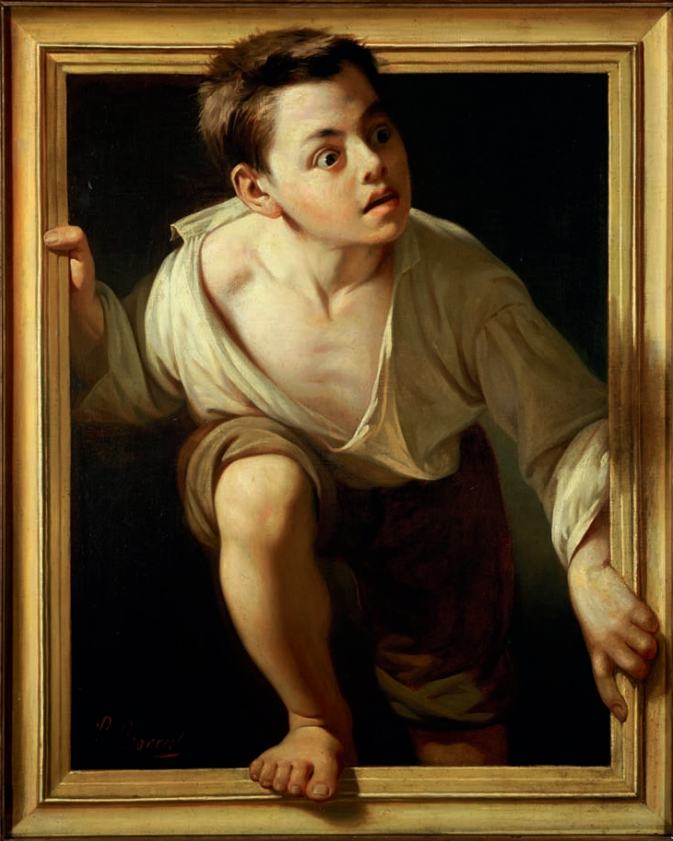
\includegraphics[width=.8\textwidth]{Borrel}
\caption{\textit{Escaping Criticism} by Pere Borrell del Caso, 1874}
\end{figure}
\end{column}
\end{columns}
\end{frame}

\begin{frame}
\begin{columns}
\begin{column}{.6\textwidth}
\begin{figure}[!h]
\centering
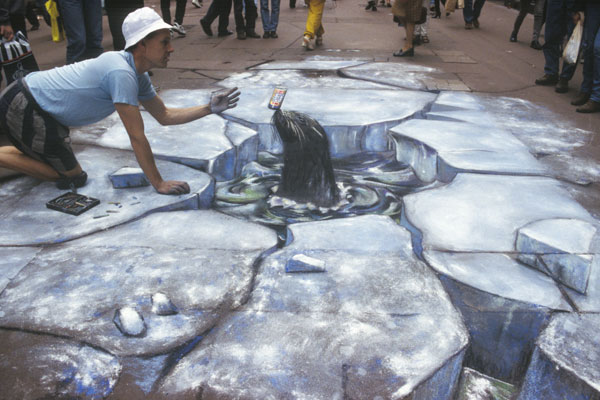
\includegraphics[width=.6\textwidth]{beever}
\end{figure}
\begin{figure}[!h]
\centering
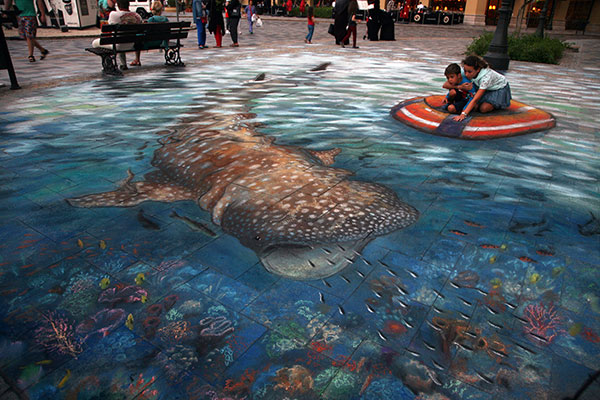
\includegraphics[width=.6\textwidth]{beever3}
\end{figure}
\end{column}
\begin{column}{.4\textwidth}
\begin{figure}[!h]
\centering
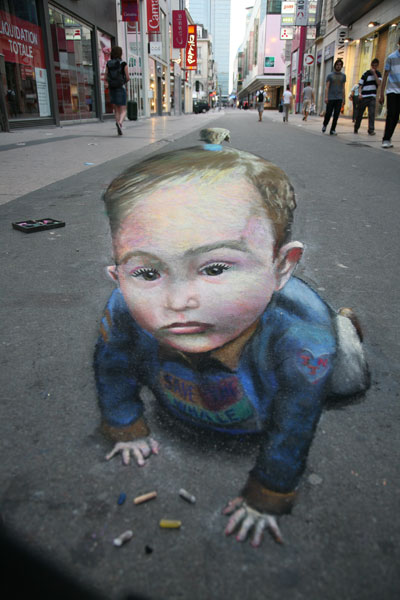
\includegraphics[width=.9\textwidth]{beever2}
\end{figure}
\end{column}
\end{columns}
\centering
\url{http://julianbeever.net/}
\end{frame}

\begin{frame}
\begin{columns}
\begin{column}{.5\textwidth}
\begin{figure}[!h]
\centering
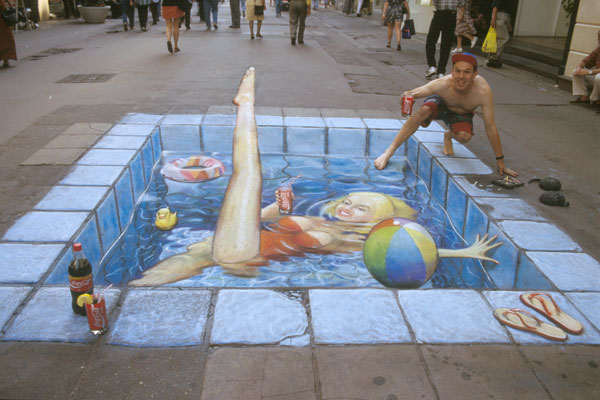
\includegraphics[width=\textwidth]{beever4}
\end{figure}
\end{column}
\begin{column}{.5\textwidth}
\begin{figure}[!h]
\centering
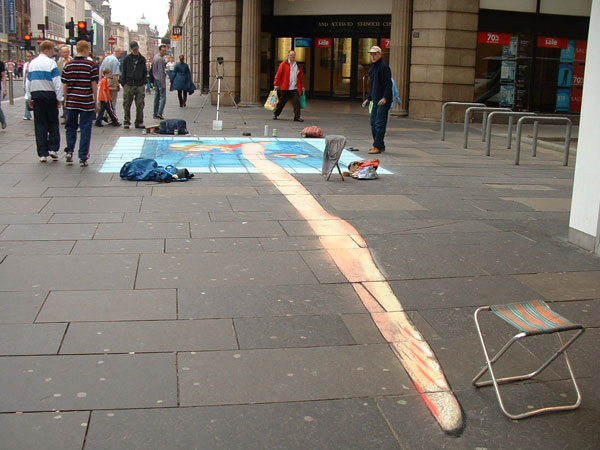
\includegraphics[width=.9\textwidth]{beever5}
\end{figure}
\end{column}
\end{columns}
\url{http://julianbeever.net/}
\end{frame}

\begin{frame}
\begin{figure}[!h]
\centering
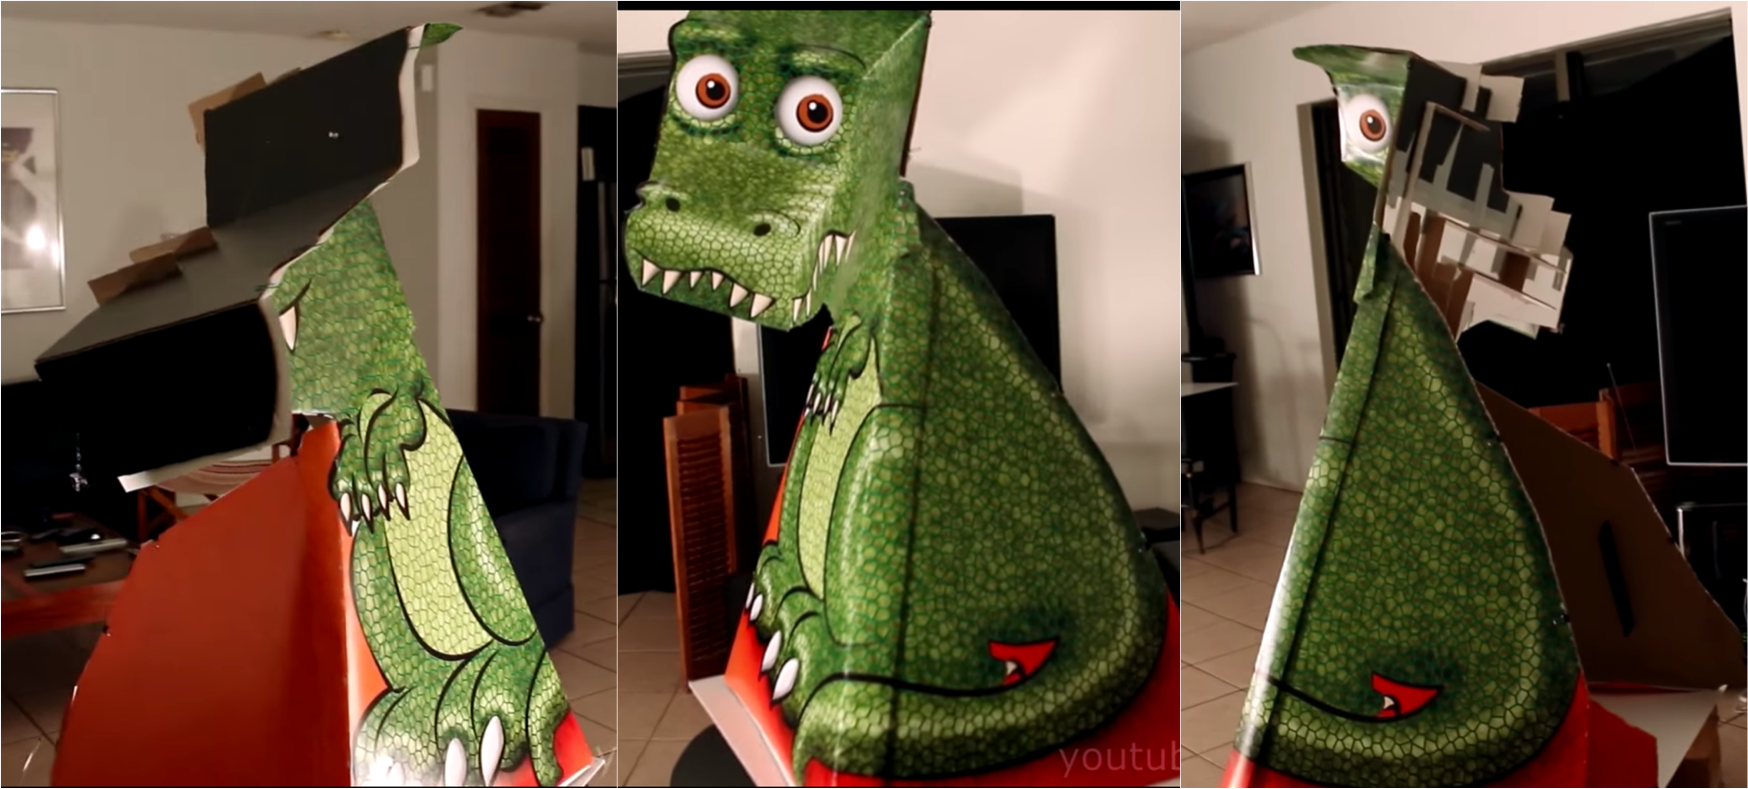
\includegraphics[width=\textwidth]{trexs}
\end{figure}
\url{https://youtu.be/A4QcyW-qTUg?list=FLBJEFWqBtSxR67zLiyi6uAg}
\end{frame}

\begin{frame}
\begin{figure}[!h]
\centering
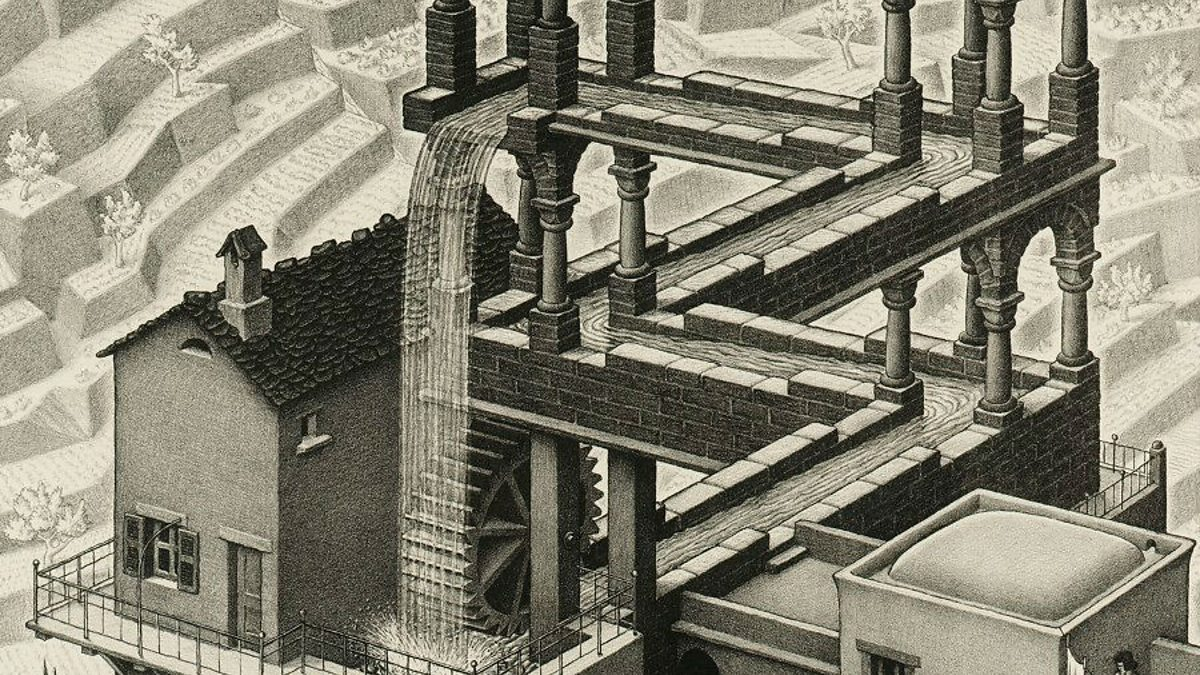
\includegraphics[width=\textwidth]{escher}
\caption{\textit{Waterfal} M. C. Escher 1961}
\end{figure}
\url{https://youtu.be/0v2xnl6LwJE}
\end{frame}

\begin{frame}
\begin{figure}[!h]
\centering
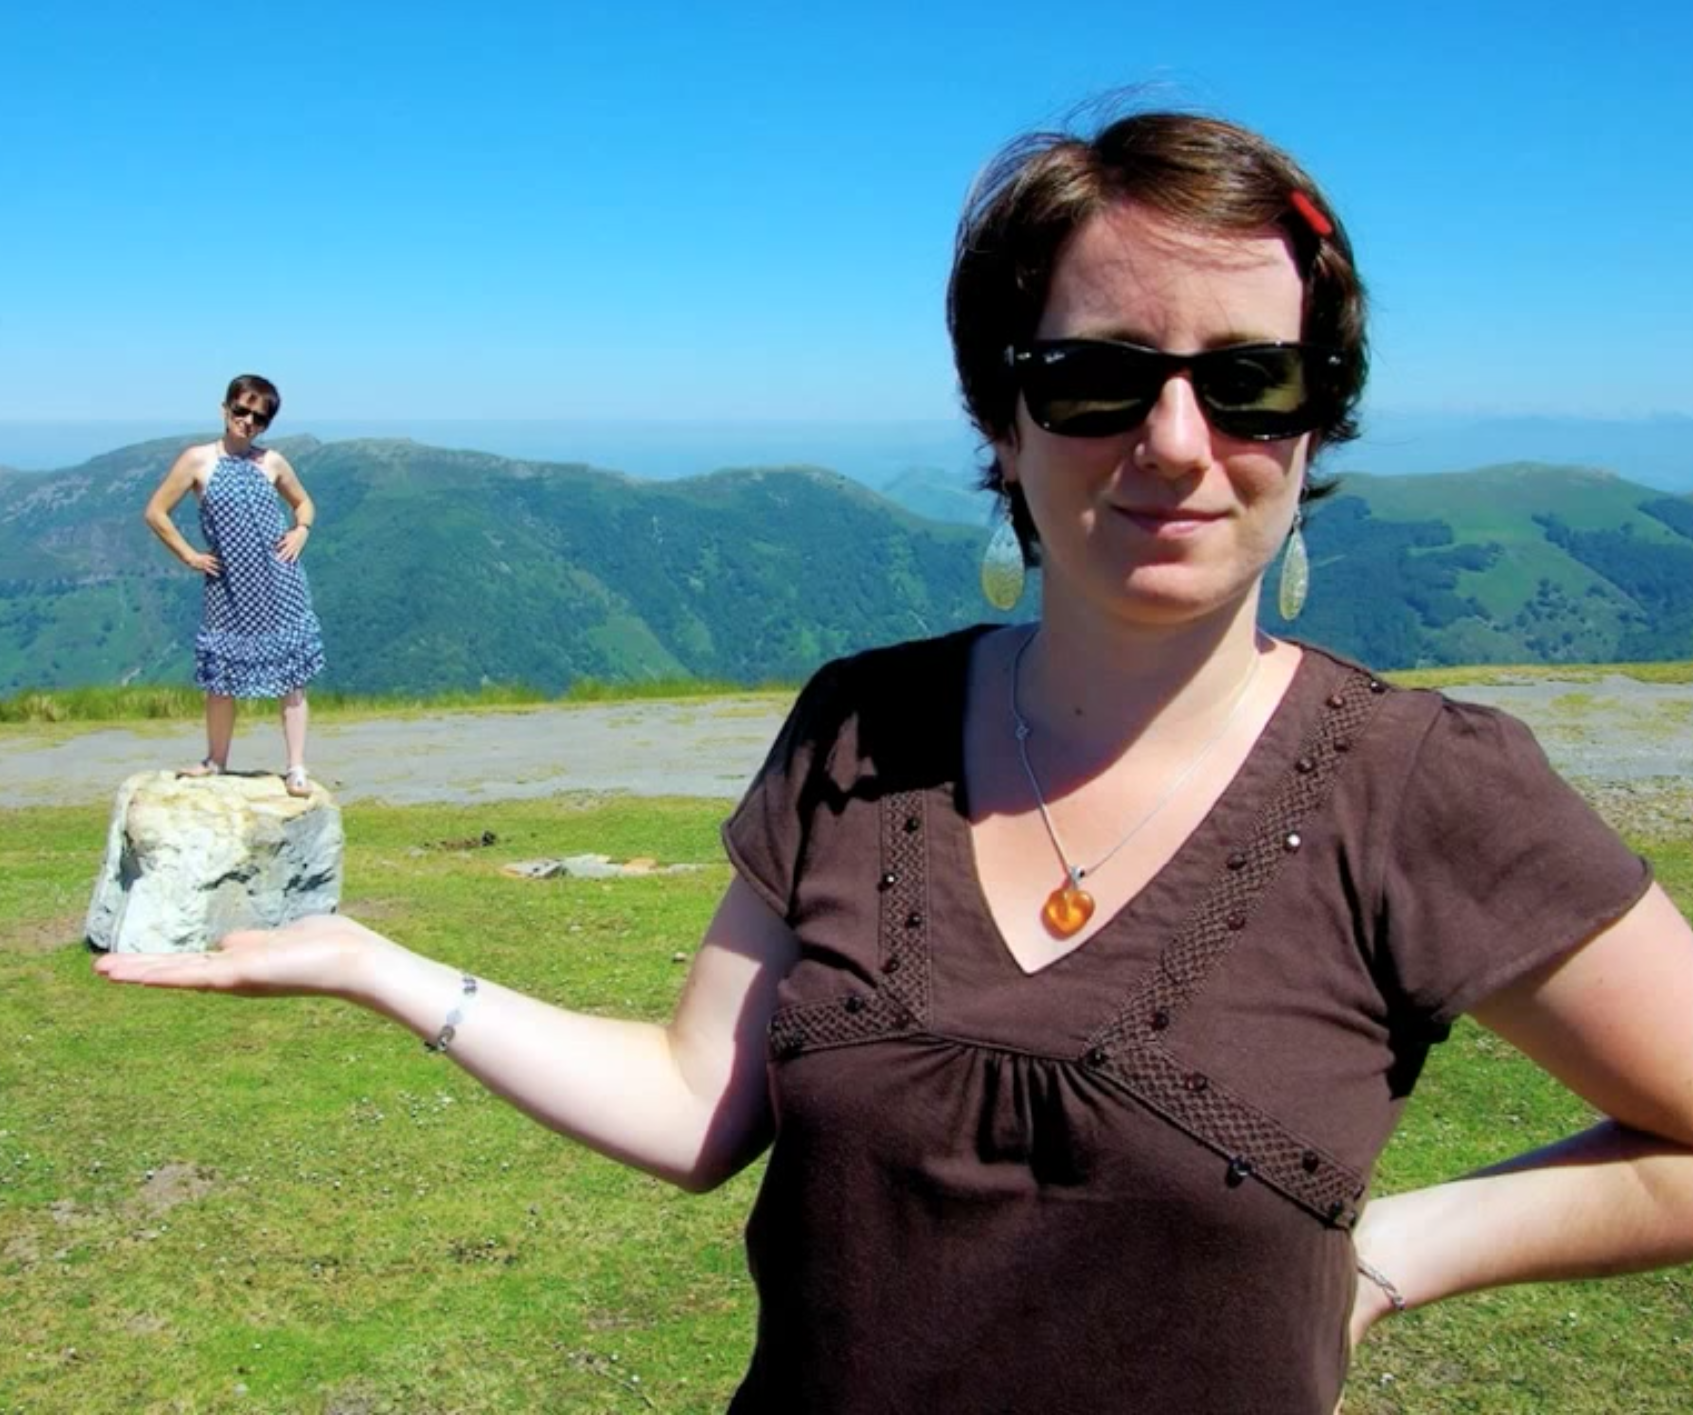
\includegraphics[width=\textwidth]{tinyFriend}
\end{figure}
\end{frame}

\begin{frame}
Specular Reflection.
Lambertian Reflection.
Retro-reflective reflection.
\end{frame}

\begin{frame}
\begin{figure}[!h]
\centering
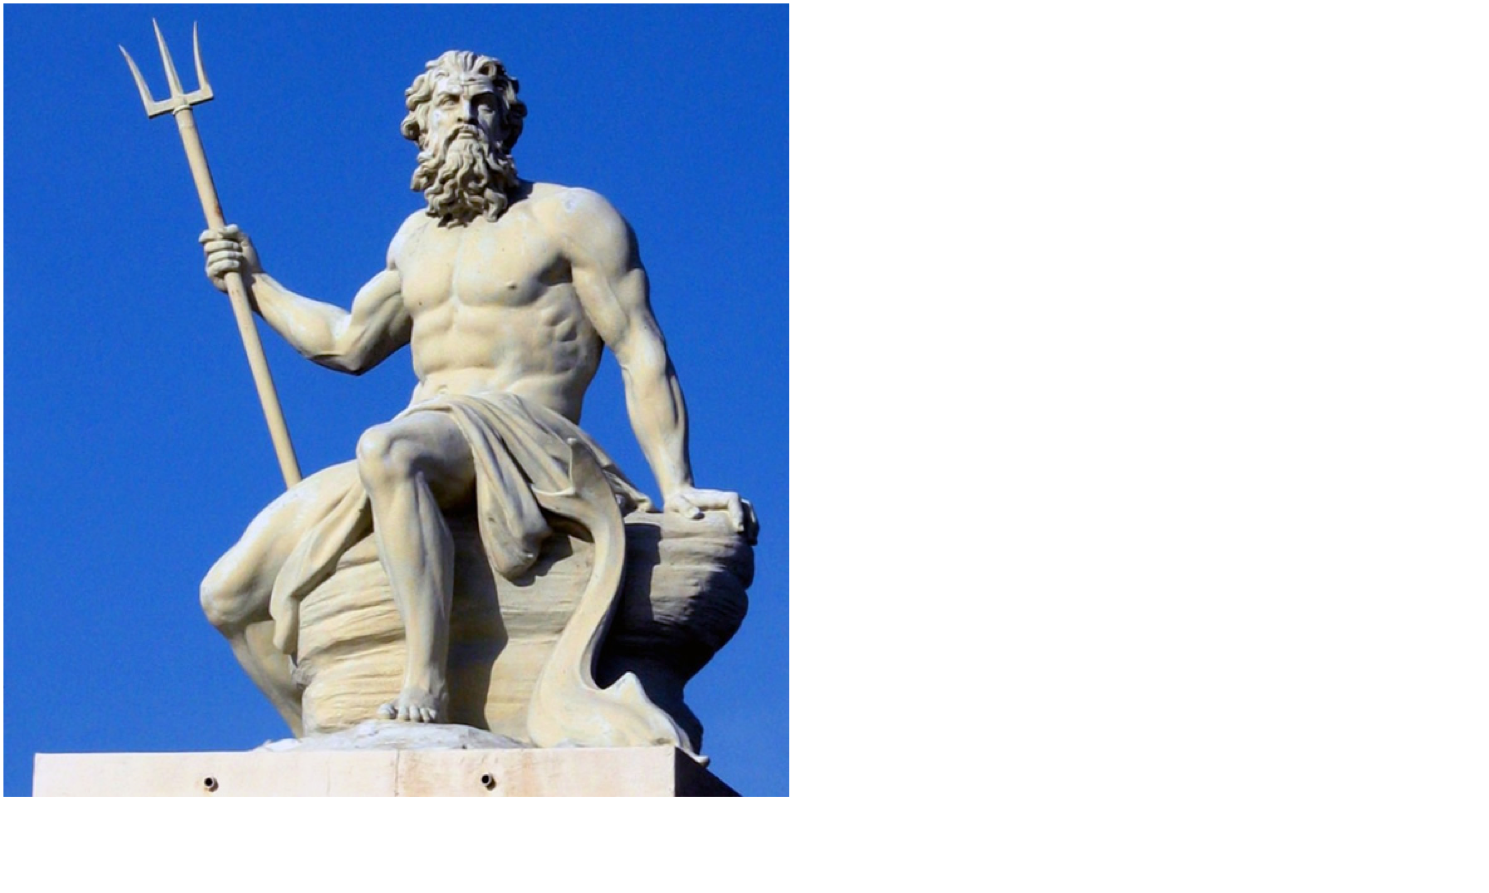
\includegraphics[width=\textwidth]{neptune1}
\end{figure}
\end{frame}

\begin{frame}
\begin{figure}[!h]
\centering
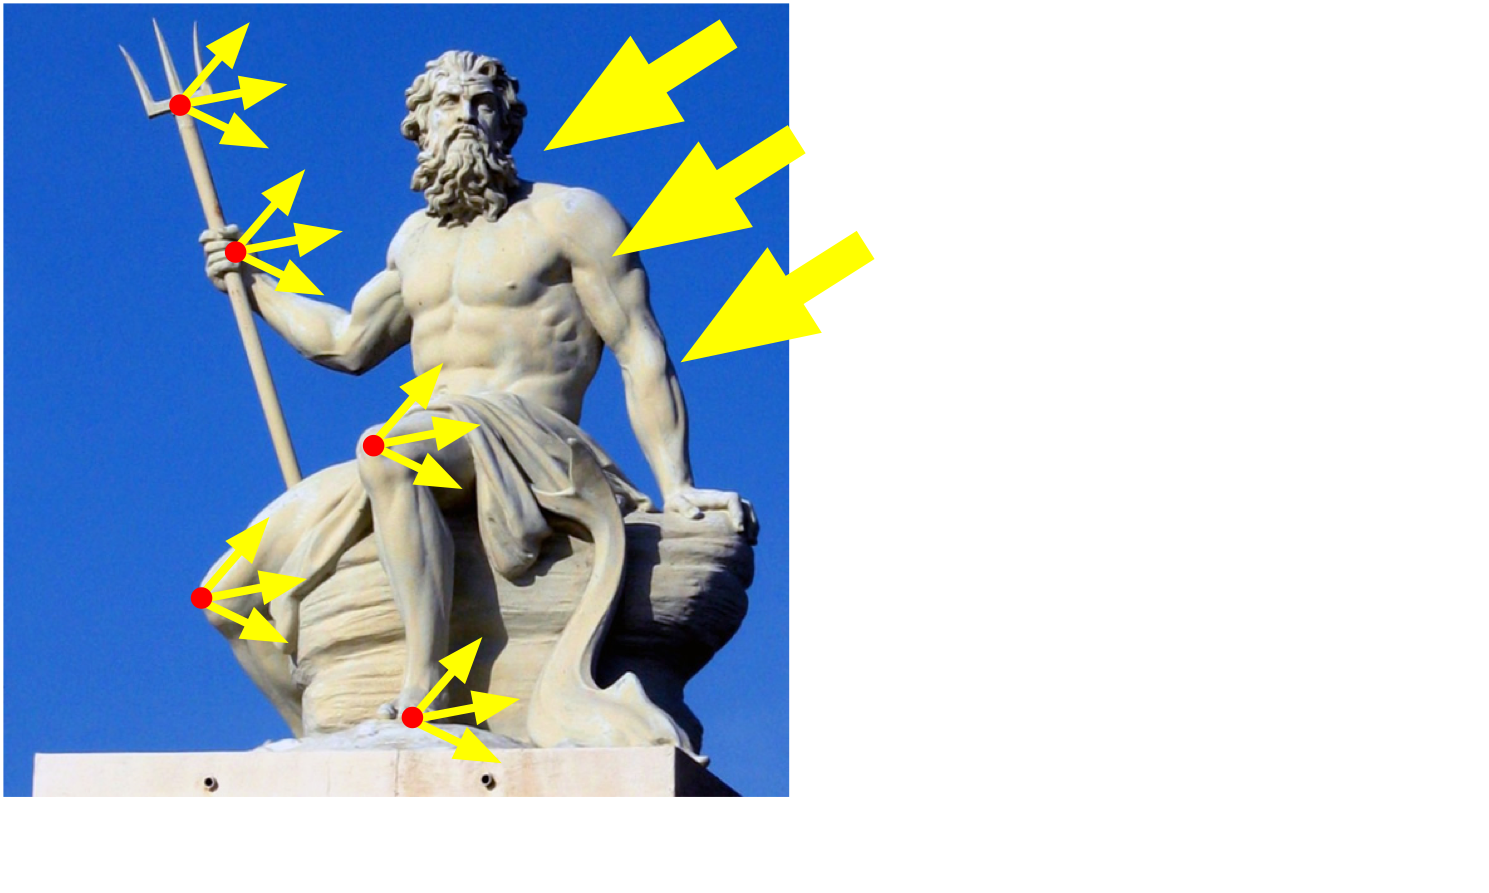
\includegraphics[width=\textwidth]{neptune2}
\end{figure}
\end{frame}

\begin{frame}
\begin{figure}[!h]
\centering
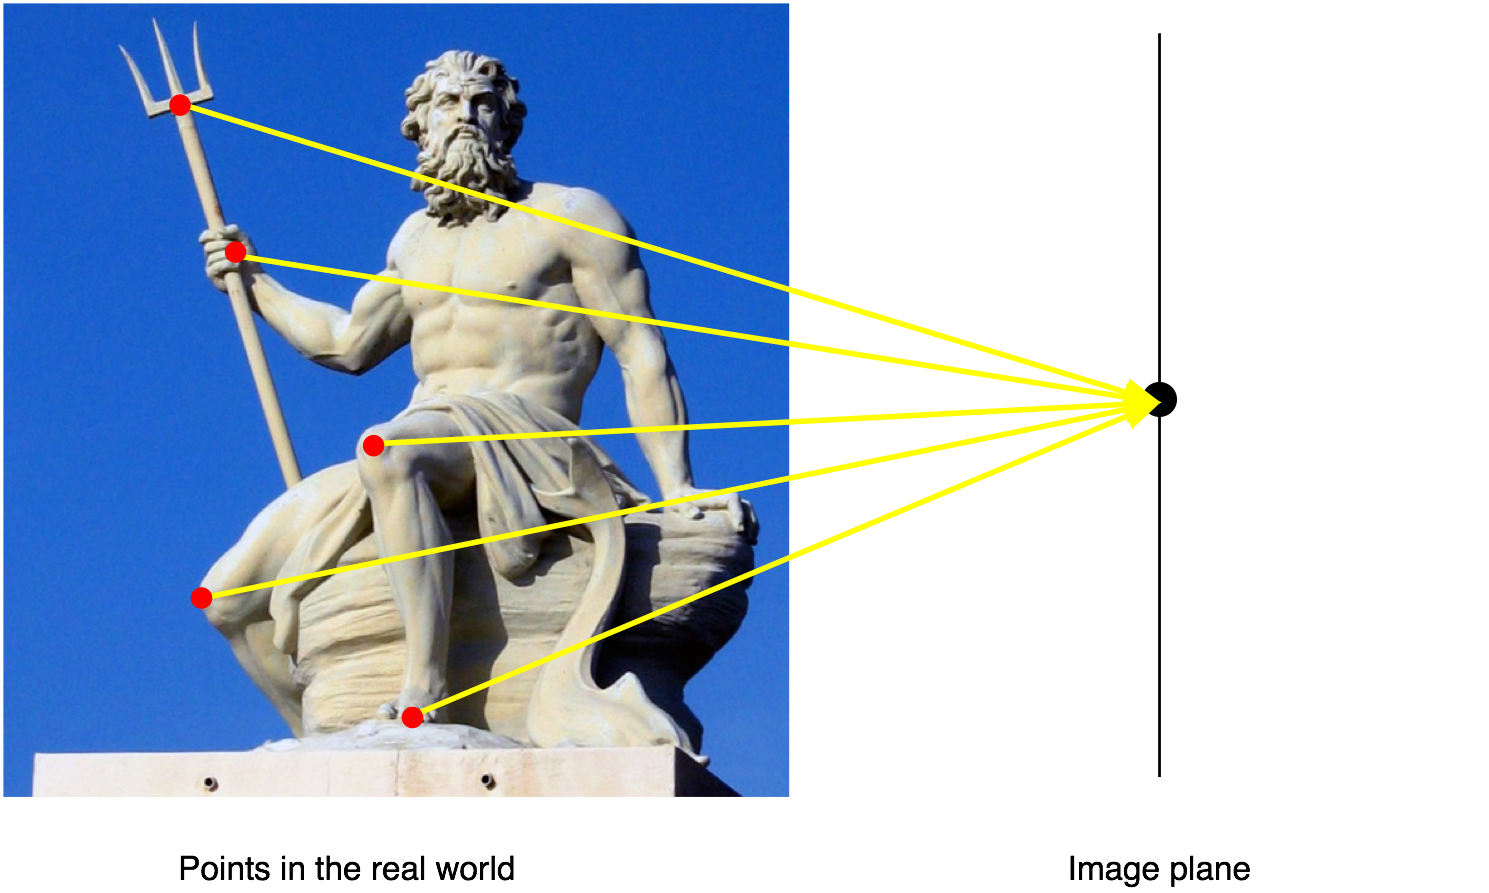
\includegraphics[width=\textwidth]{neptune3}
\end{figure}
\end{frame}

\begin{frame}
\begin{figure}[!h]
\centering
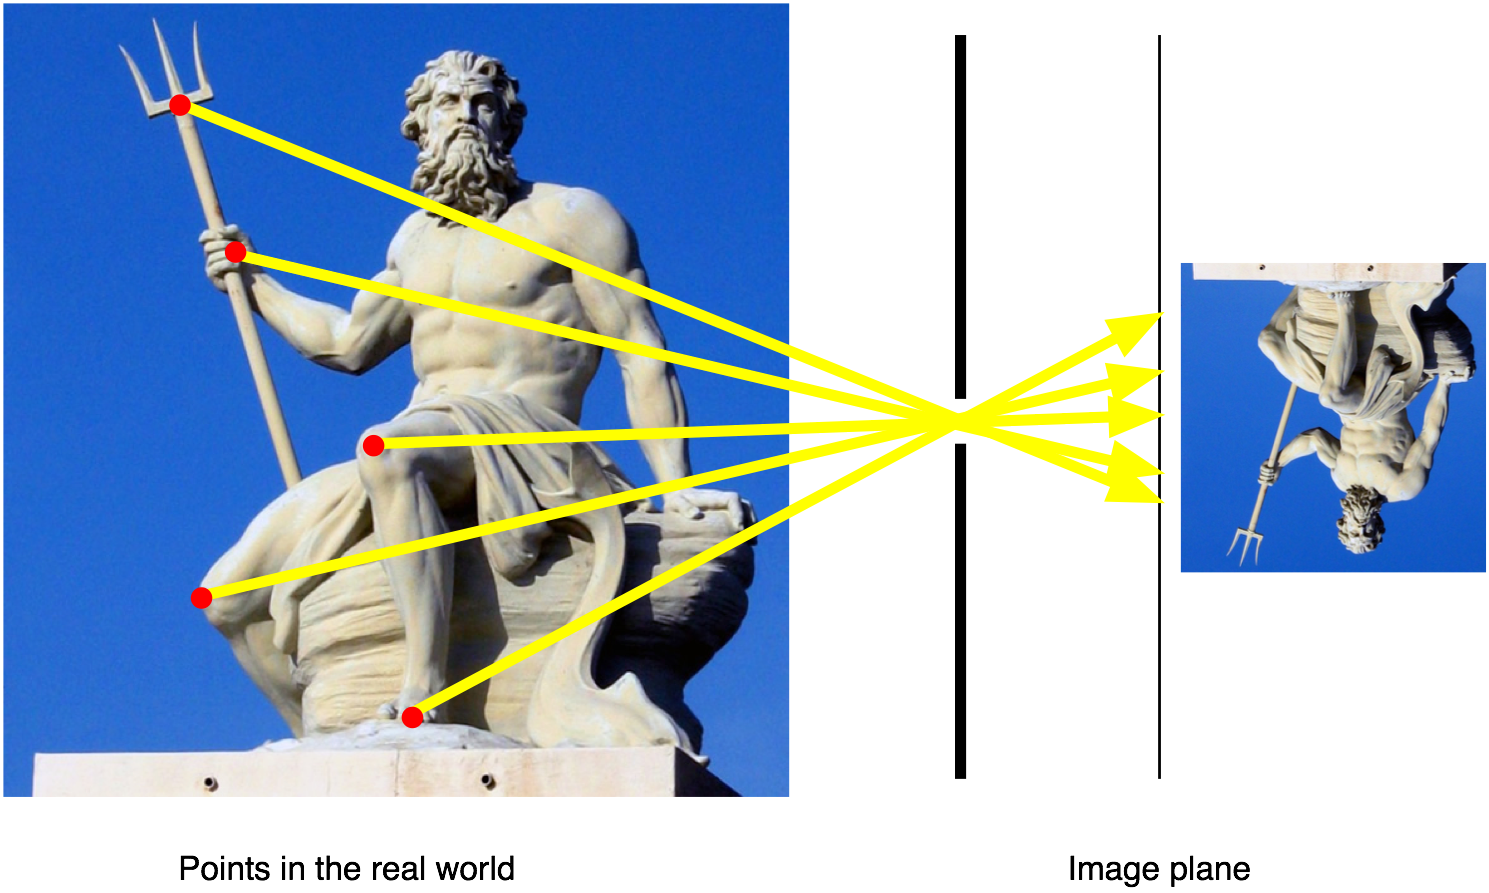
\includegraphics[width=\textwidth]{neptune4}
\end{figure}
\end{frame}

\begin{frame}
\frametitle{Pinhole images}
\begin{figure}[!h]
\centering
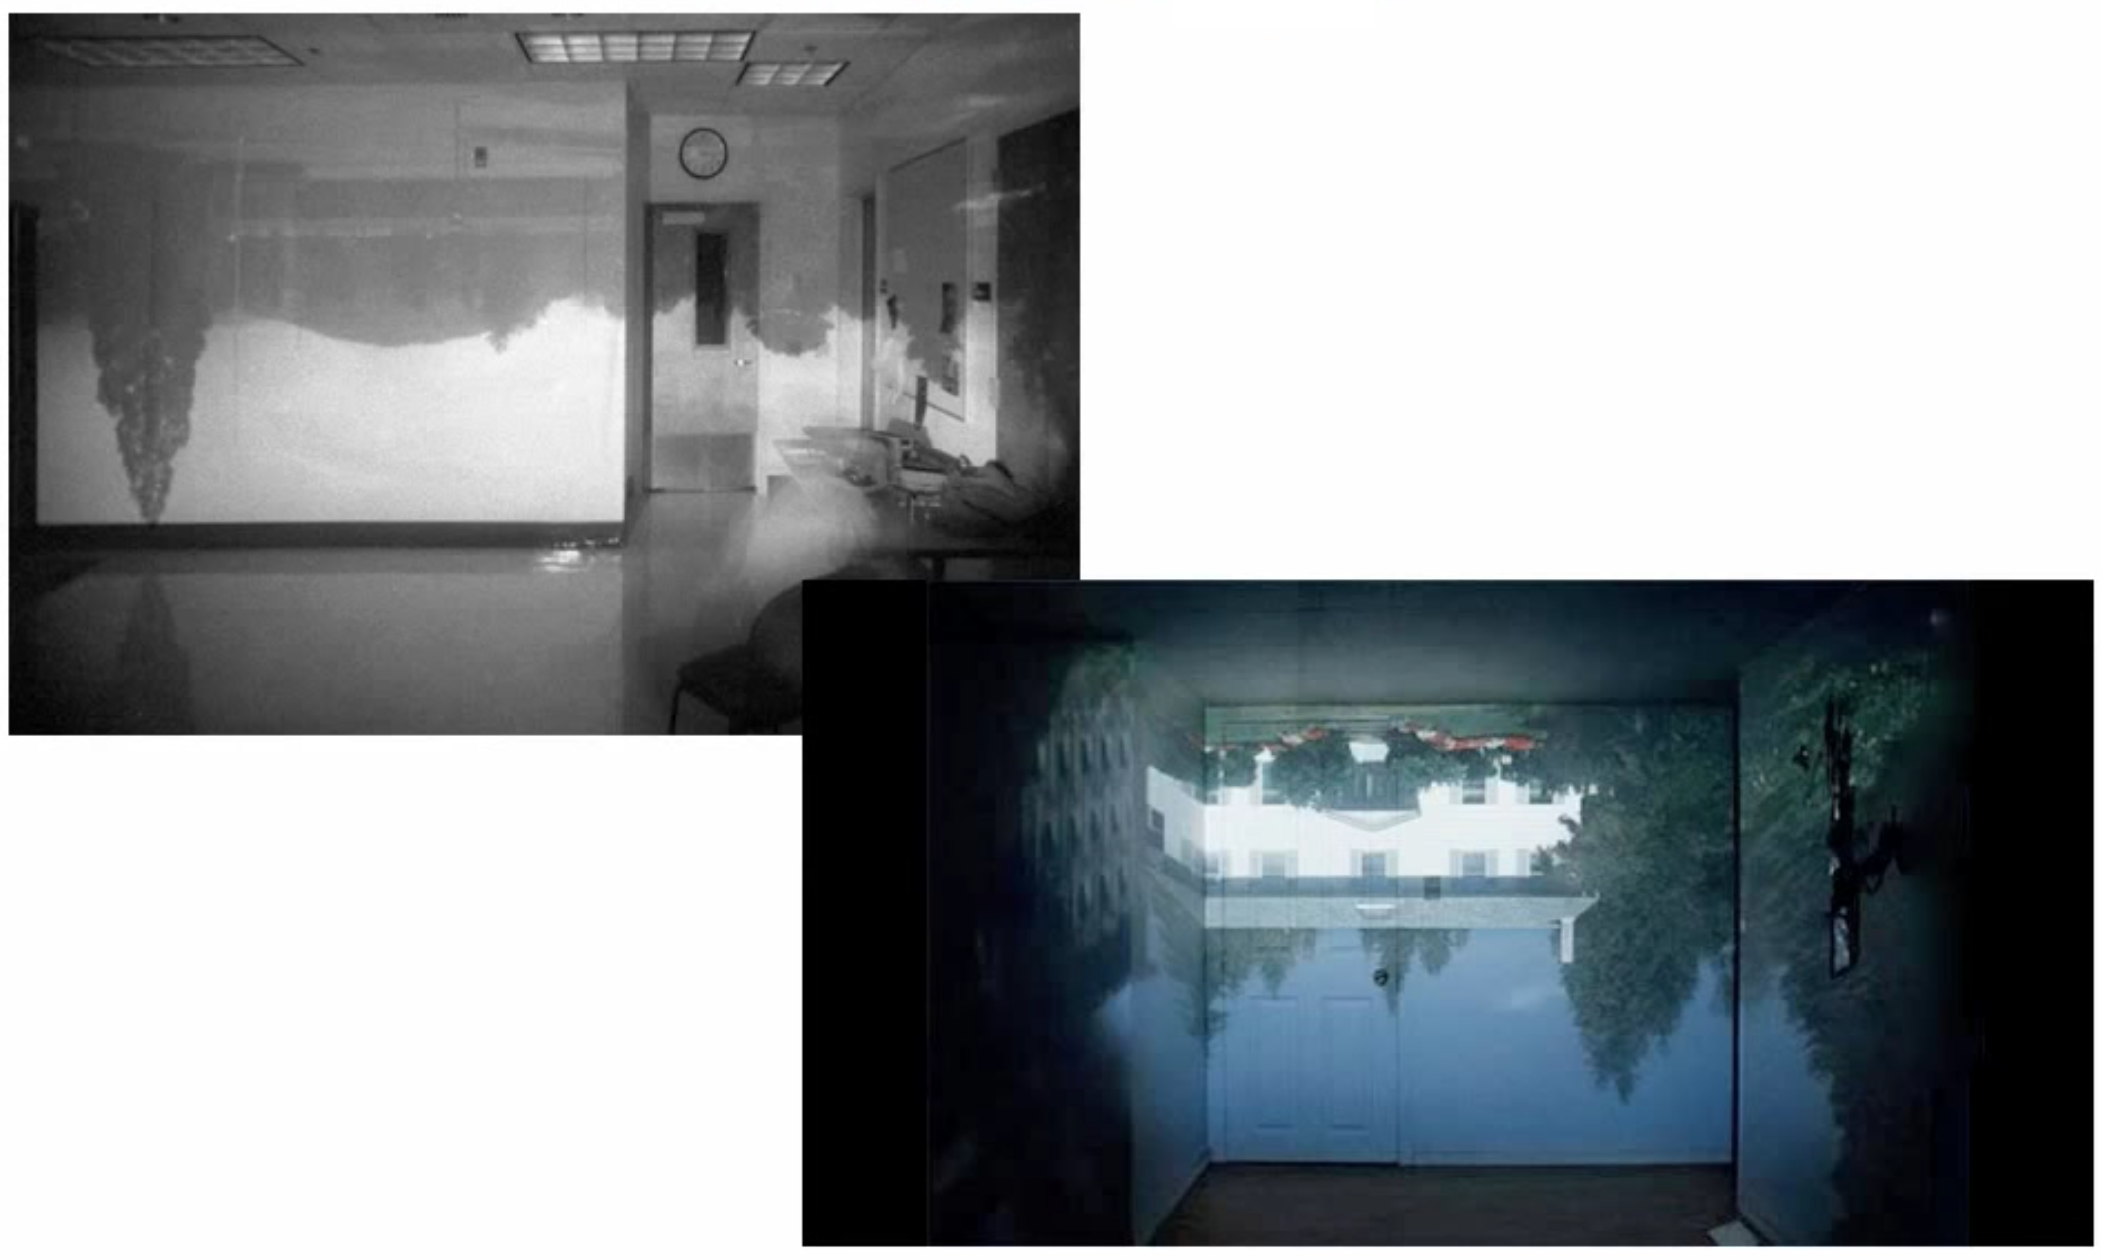
\includegraphics[width=\textwidth]{pinholeExamples}
\end{figure}
\end{frame}

\begin{frame}
\frametitle{The world's largest pinhole camera}
\begin{figure}[!h]
\centering
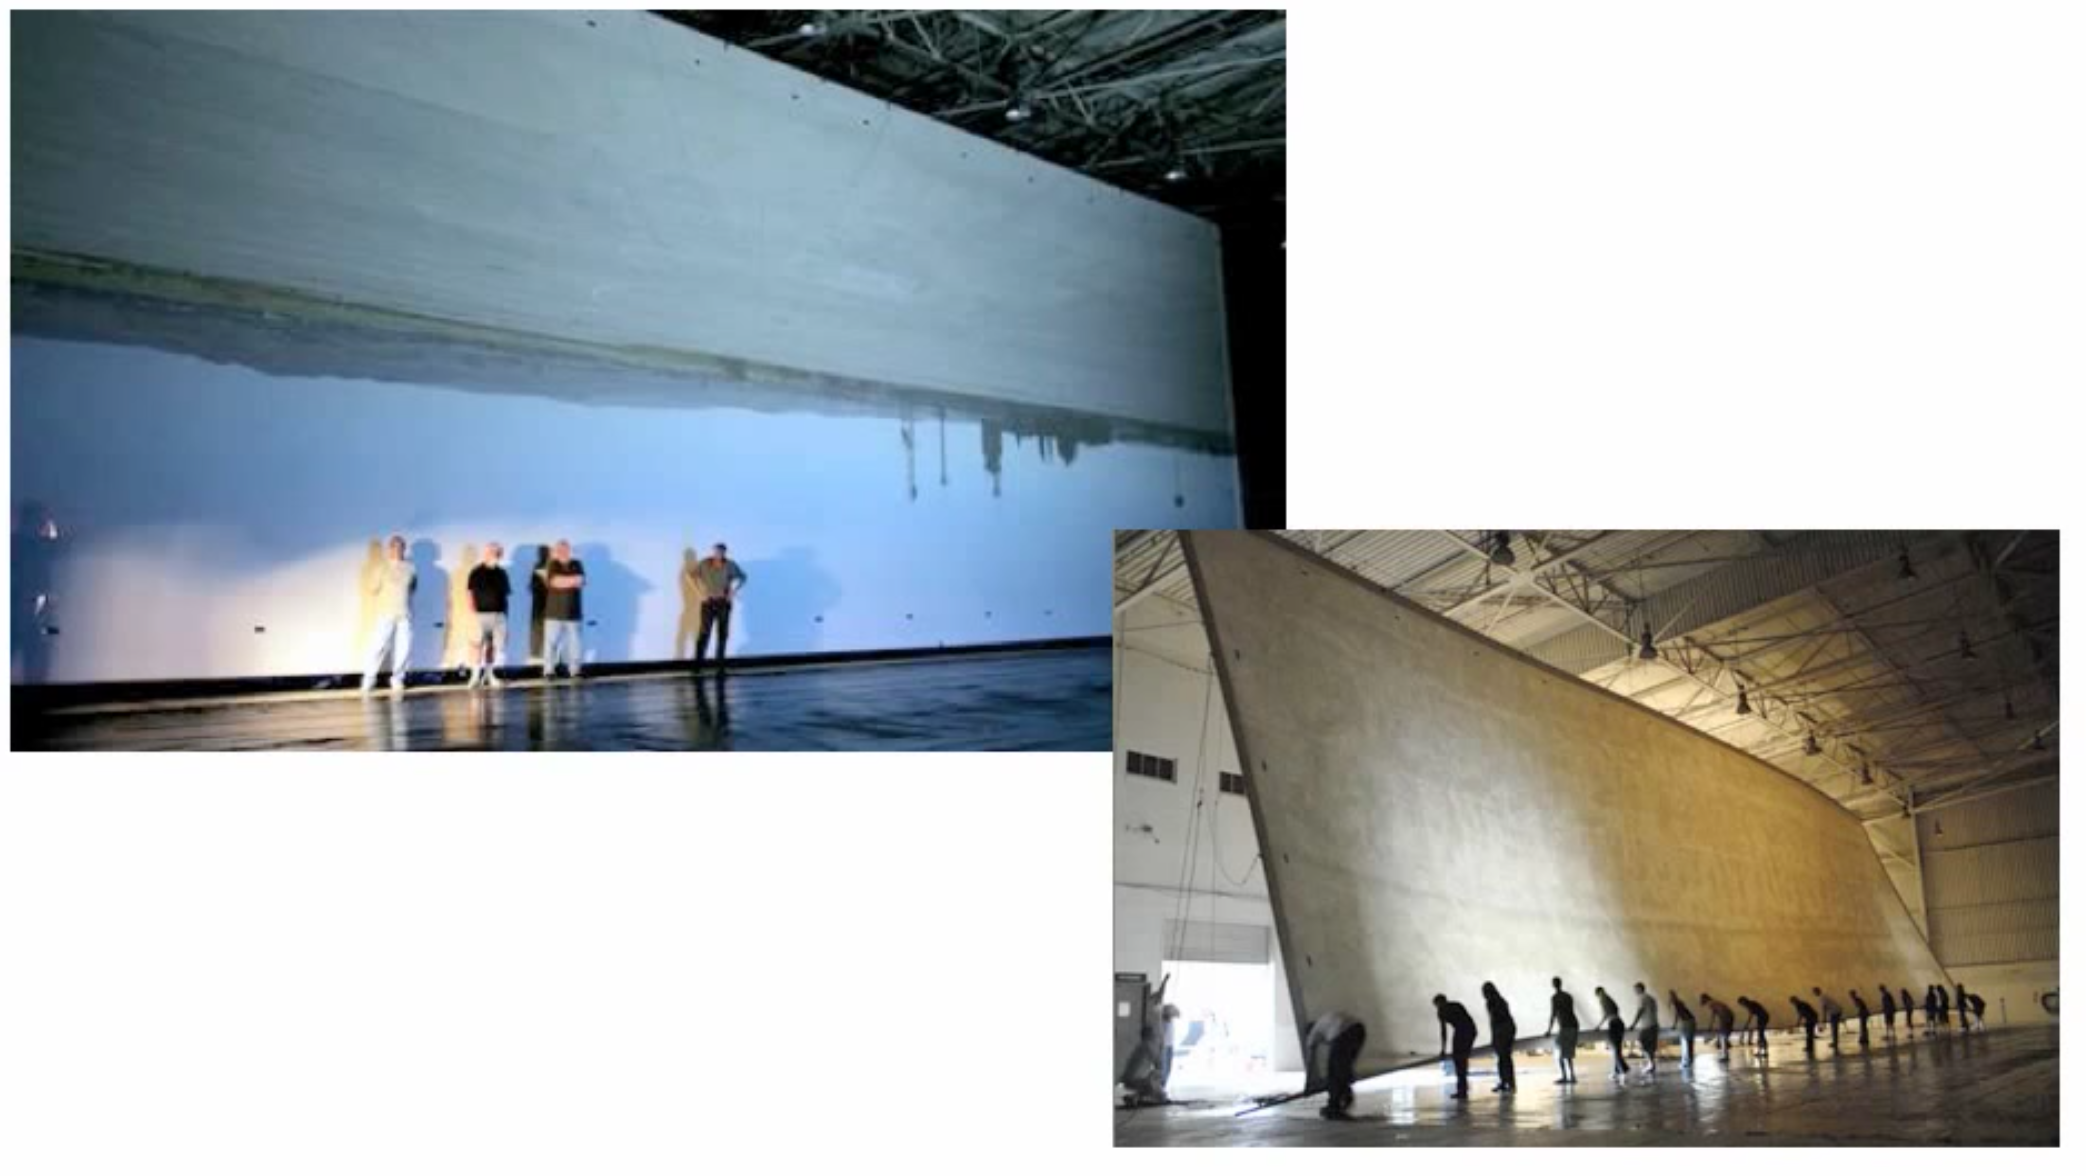
\includegraphics[width=.8\textwidth]{pinholeExamples2}
\end{figure}
\url{http://www.legacyphotoproject.com/}
\end{frame}

\begin{frame}
\frametitle{The world's largest pinhole camera}
\begin{figure}[!h]
\centering
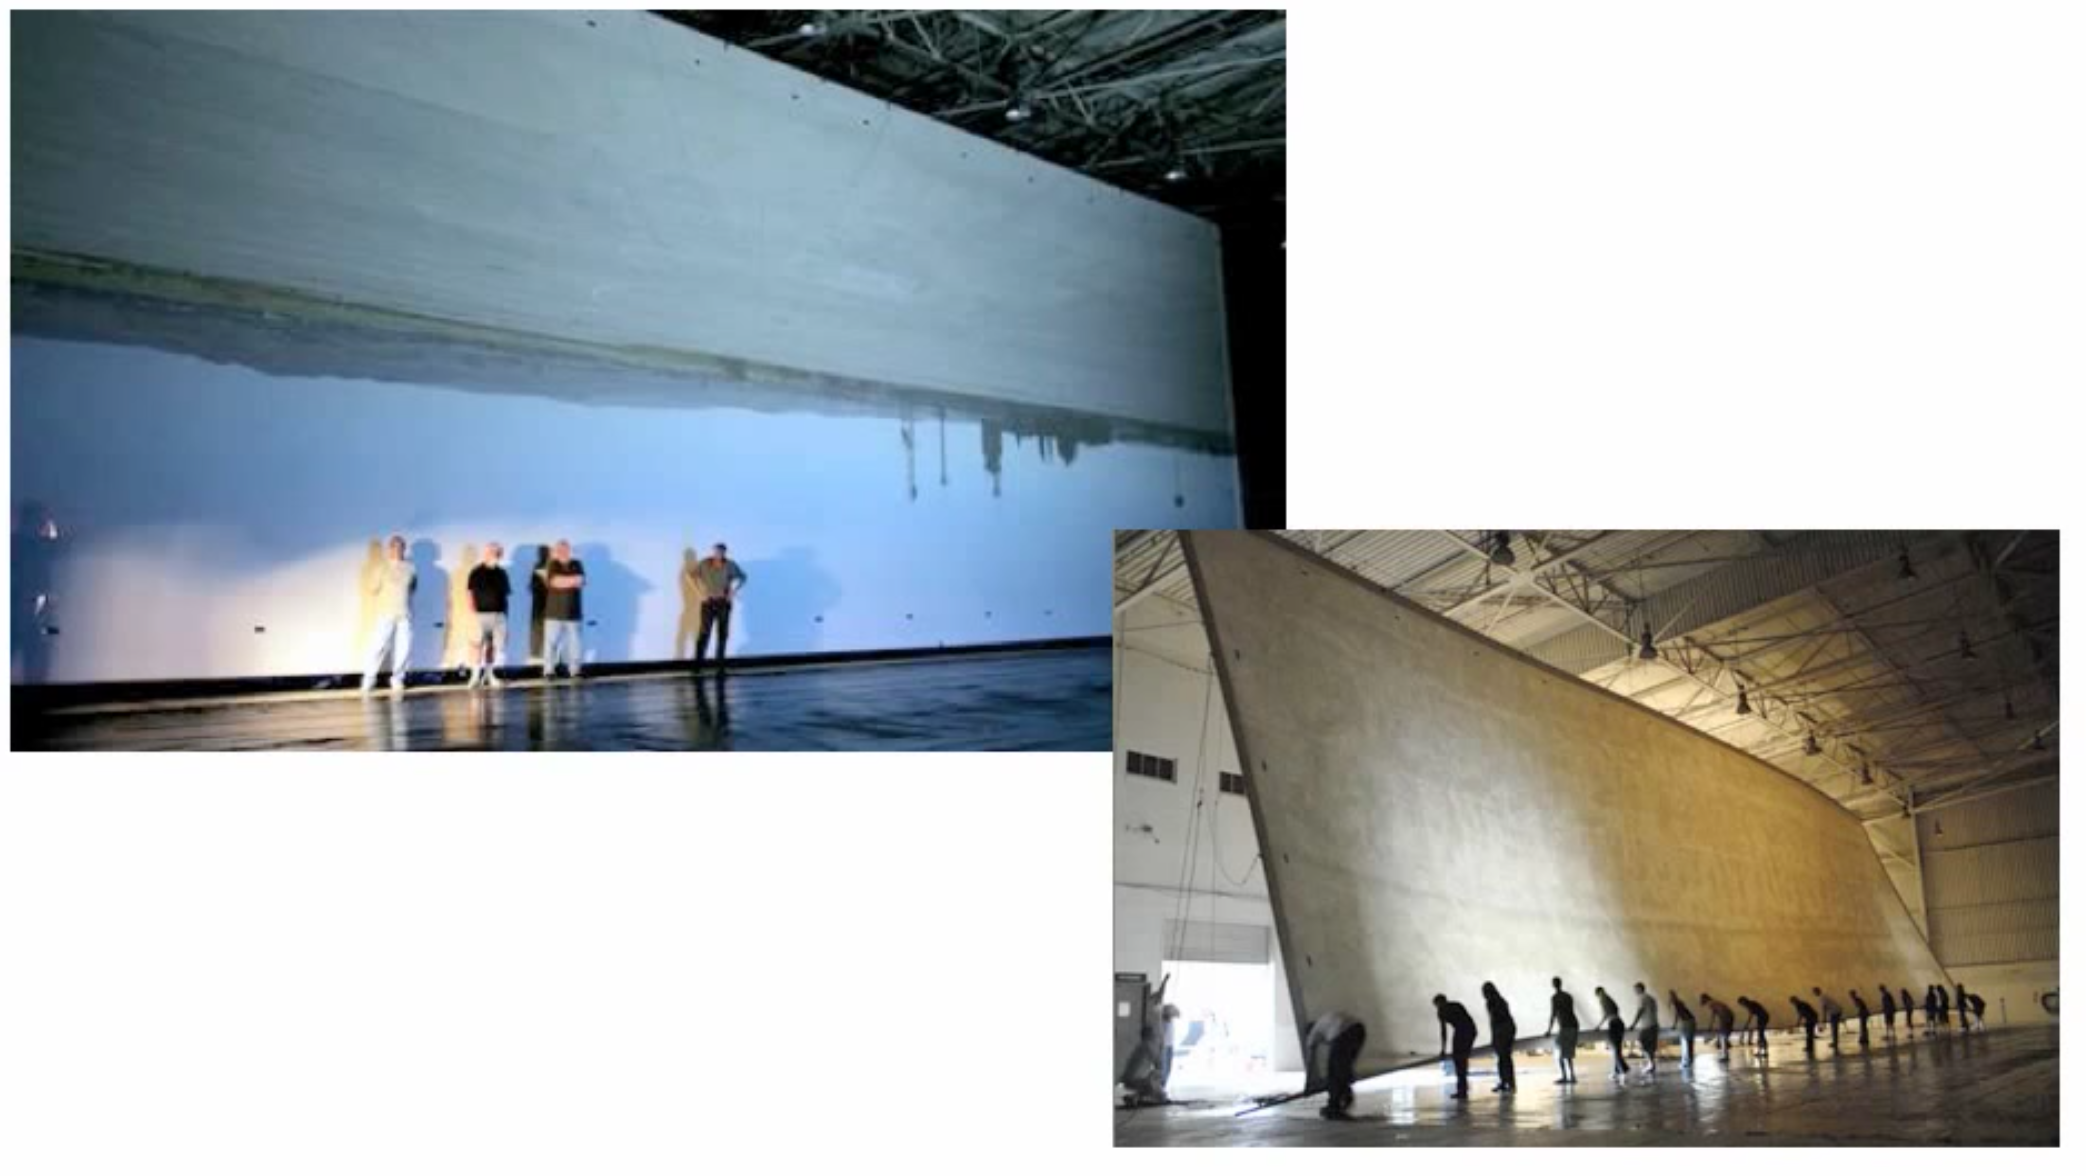
\includegraphics[width=.5\textwidth]{pinholeExamples2}
\end{figure}
\url{http://www.legacyphotoproject.com/}
\begin{itemize}
\item No lenses.
\item Long exposure.
\item Cloth with light-sensitive chemicals.
\end{itemize}
\end{frame}

\begin{frame}
\begin{figure}[!h]
\centering
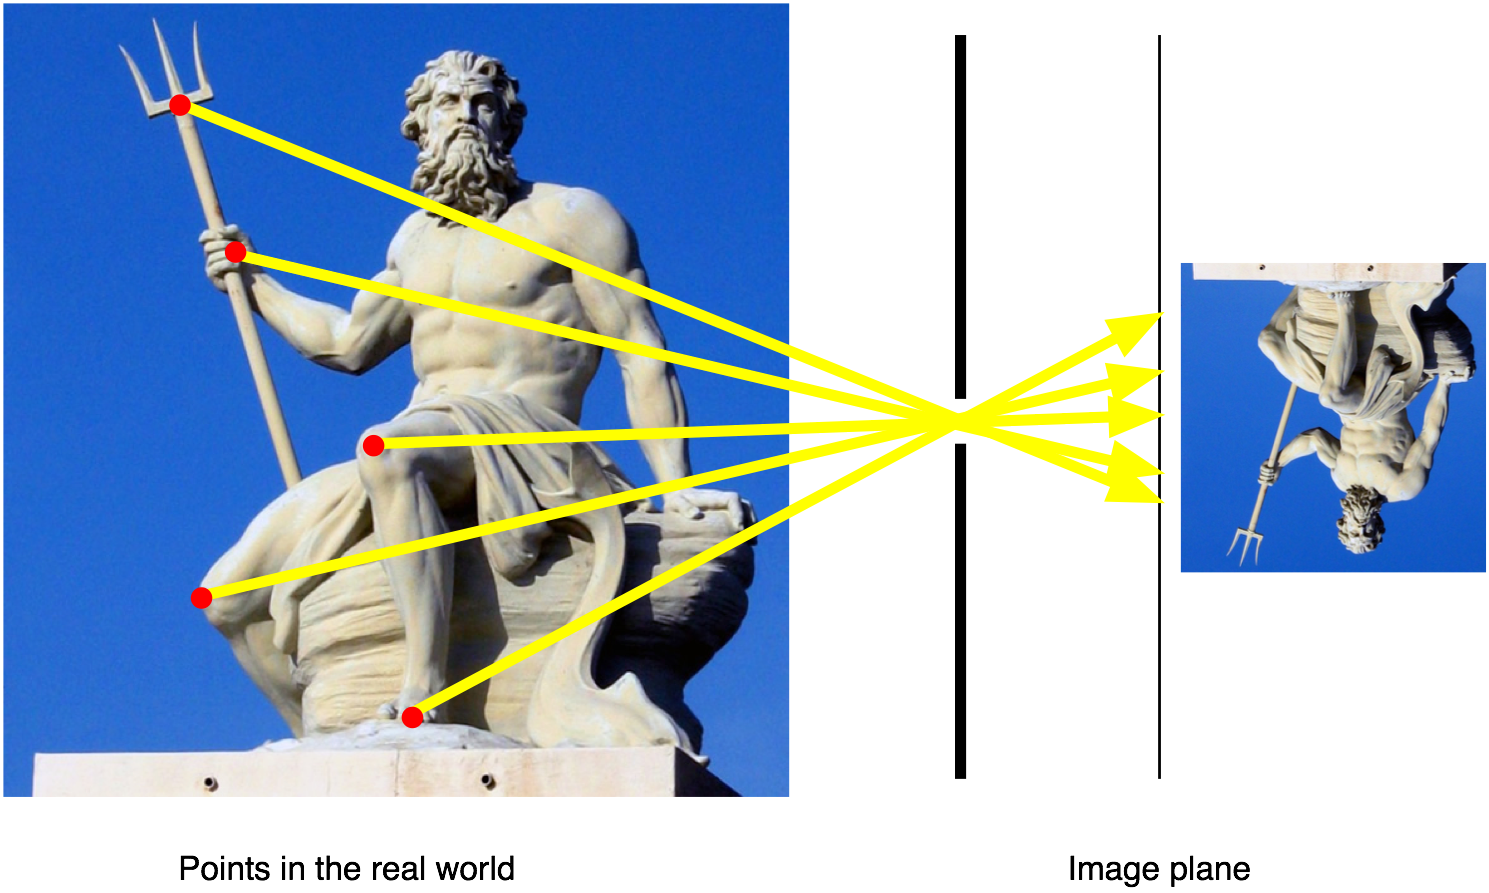
\includegraphics[width=\textwidth]{neptune4}
\end{figure}
\end{frame}

\begin{frame}
\begin{figure}[!h]
\centering
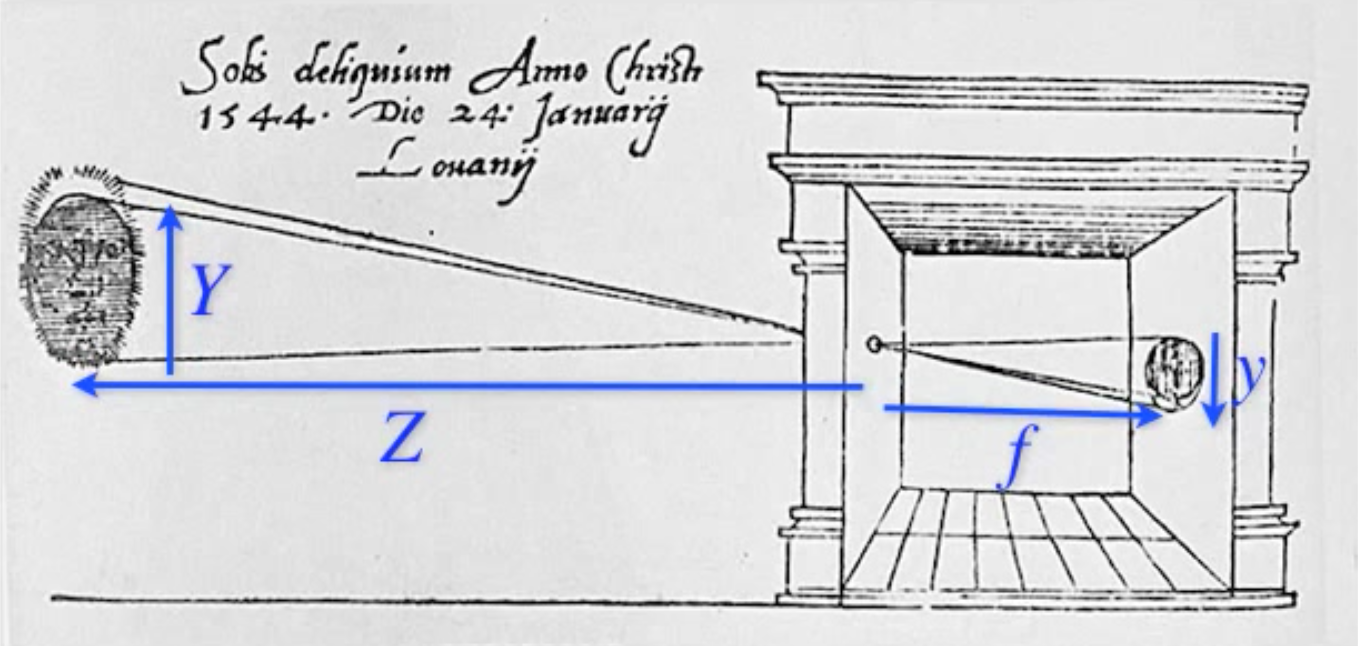
\includegraphics[width=\textwidth]{imForm}
\end{figure}
\[
\dfrac{Y}{Z} = \dfrac{y}{f}
\]
\end{frame}

\begin{frame}
\begin{figure}[!h]
\centering
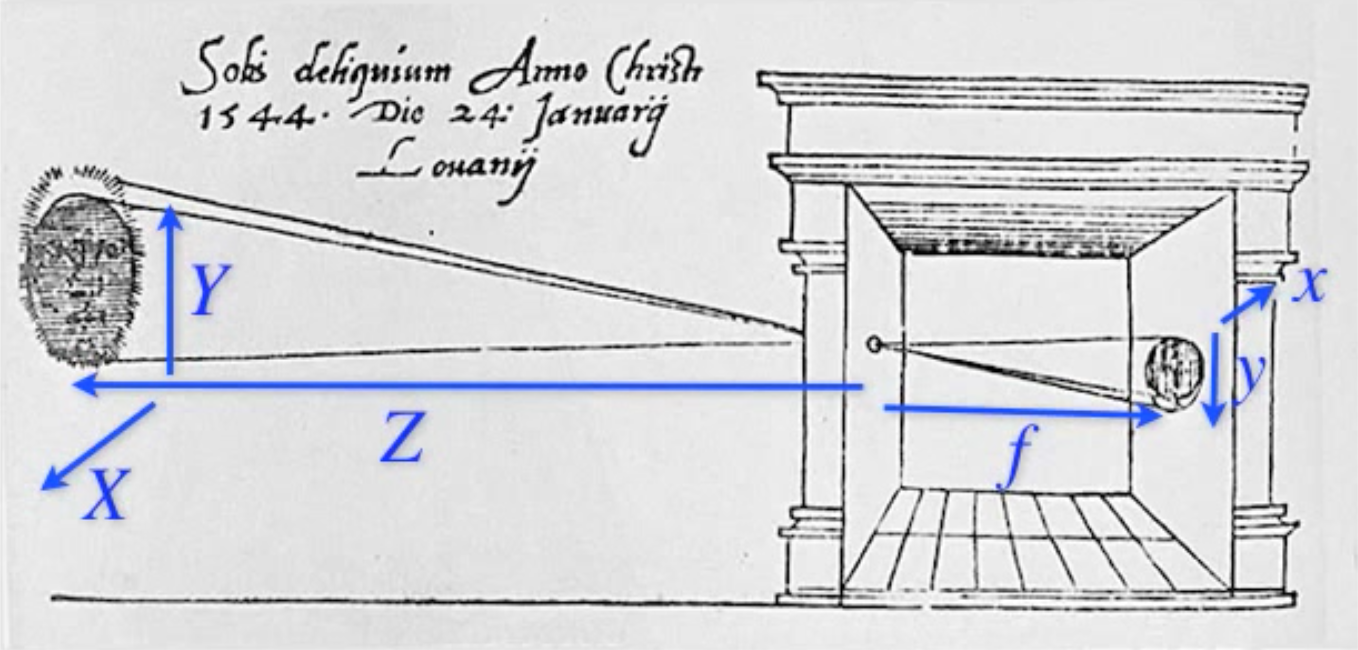
\includegraphics[width=\textwidth]{imForm2}
\end{figure}
\[
x=f\dfrac{X}{Z},\ y=f\dfrac{Y}{Z}
\]
\[
\mathbb{R}^{3} \rightarrow \mathbb{R}^{2}
\]
\end{frame}

\begin{frame}
\begin{figure}[!h]
\centering
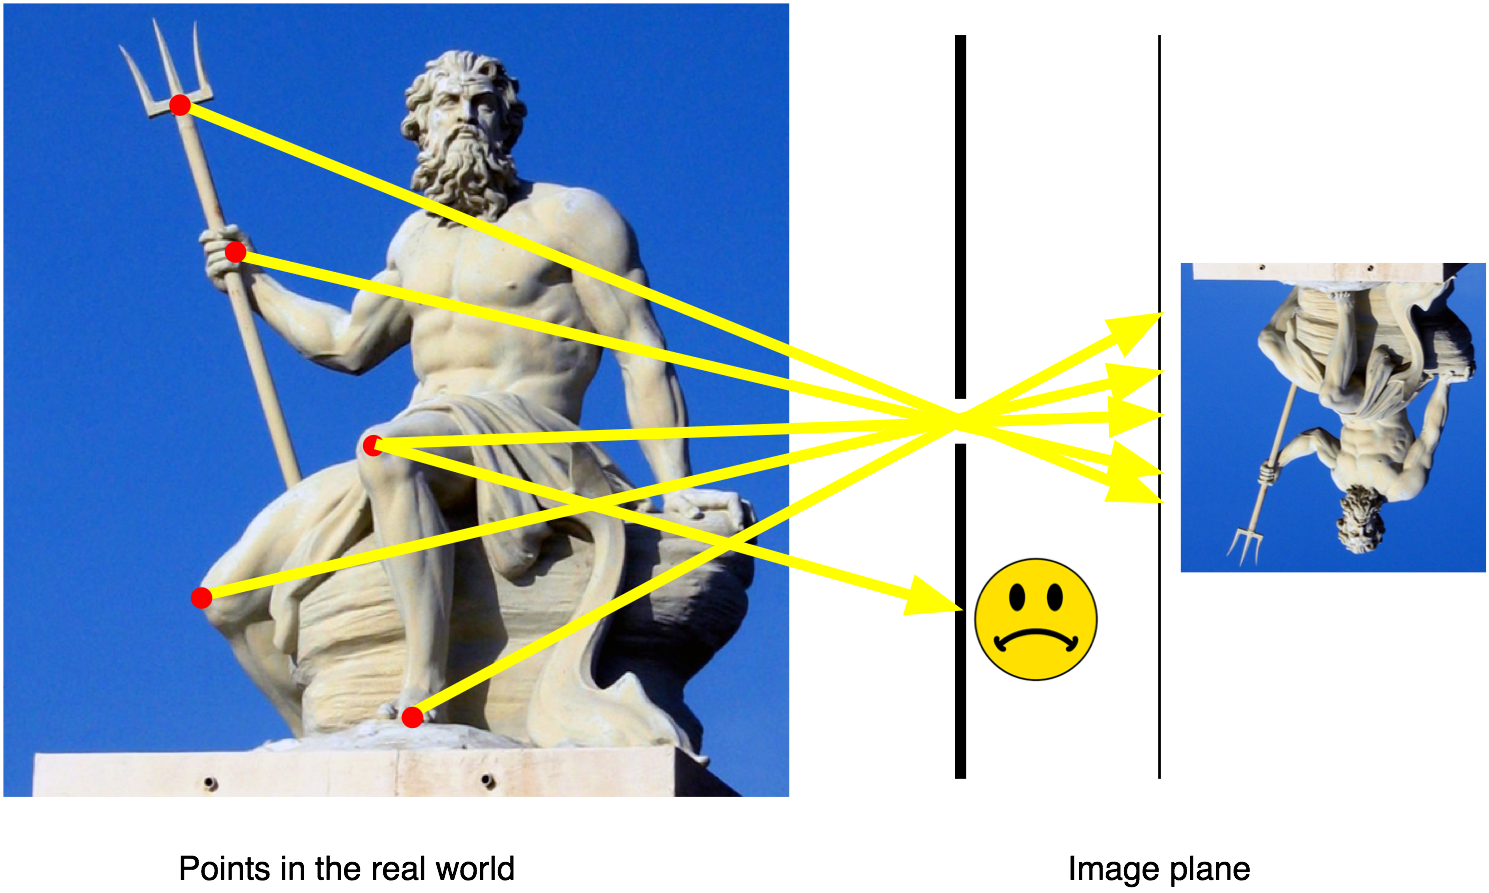
\includegraphics[width=\textwidth]{neptune5}
\end{figure}
\end{frame}

\begin{frame}
\frametitle{Use lens to capture more light}
\begin{figure}[!h]
\centering
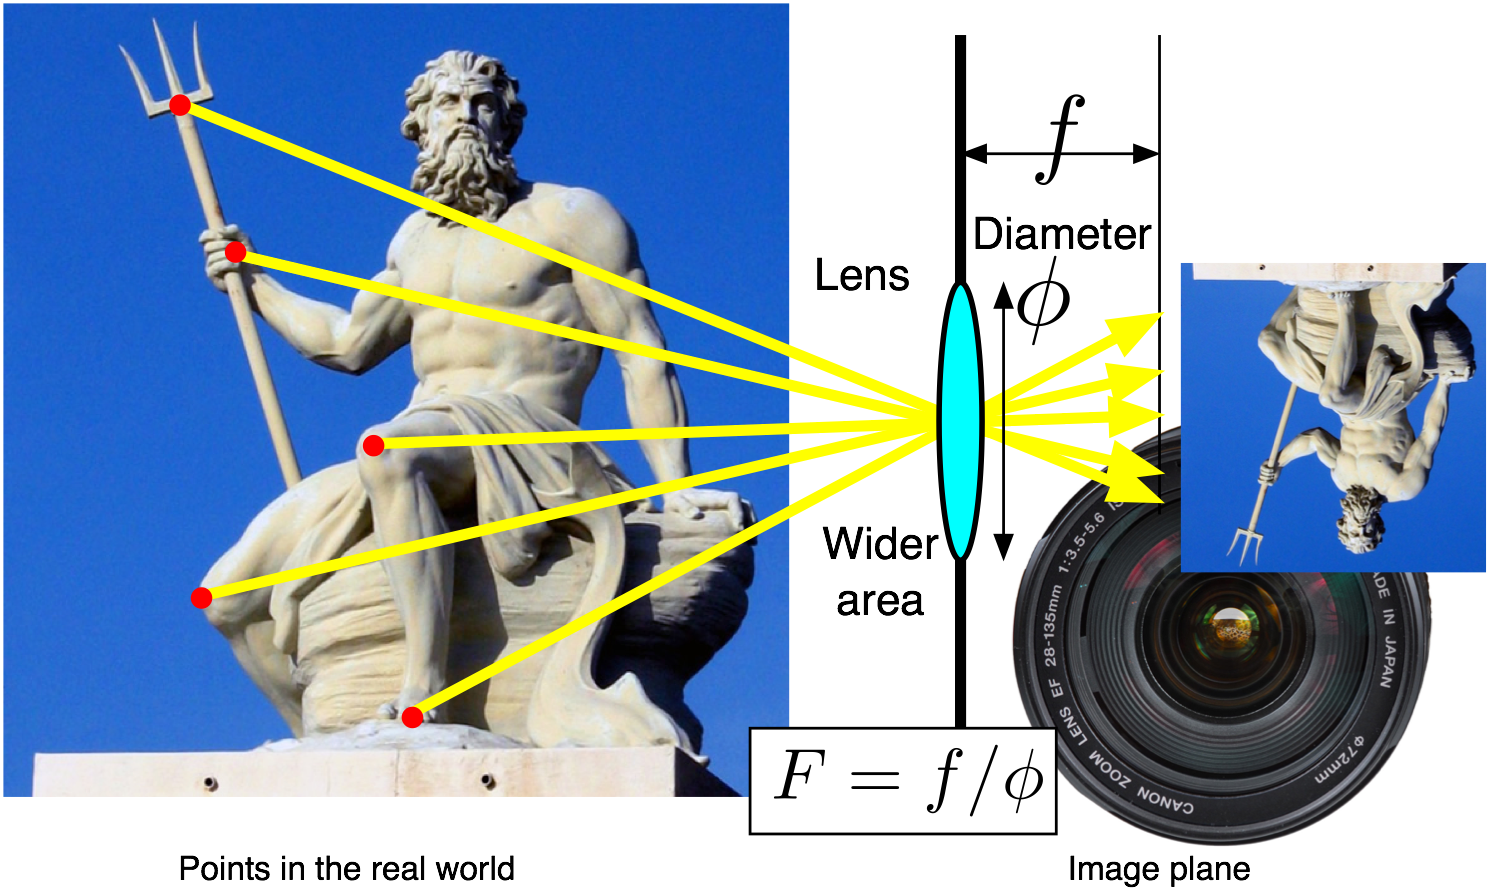
\includegraphics[width=\textwidth]{neptune6}
\end{figure}
\end{frame}

\begin{frame}
\frametitle{Use lens to capture more light}
\begin{figure}[!h]
\centering
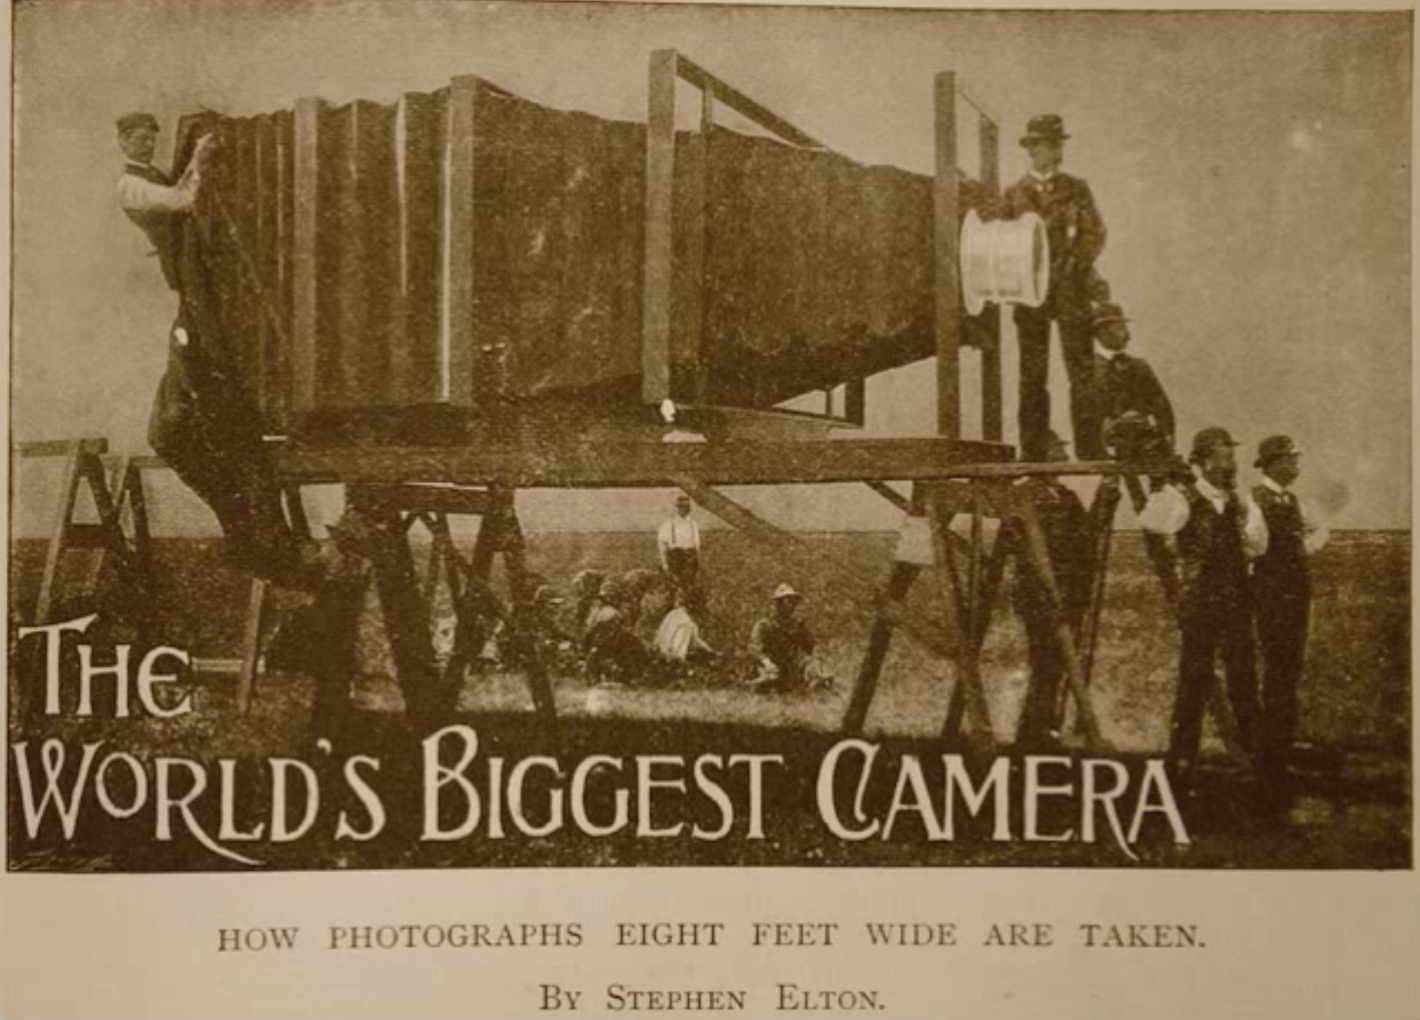
\includegraphics[width=.7\textwidth]{lawrence}
\caption{George Lawrence 1900}
\end{figure}
\end{frame}

\section{Thin lens model}

\begin{frame}
\frametitle{Thin lens model}
\begin{figure}[!h]
\centering
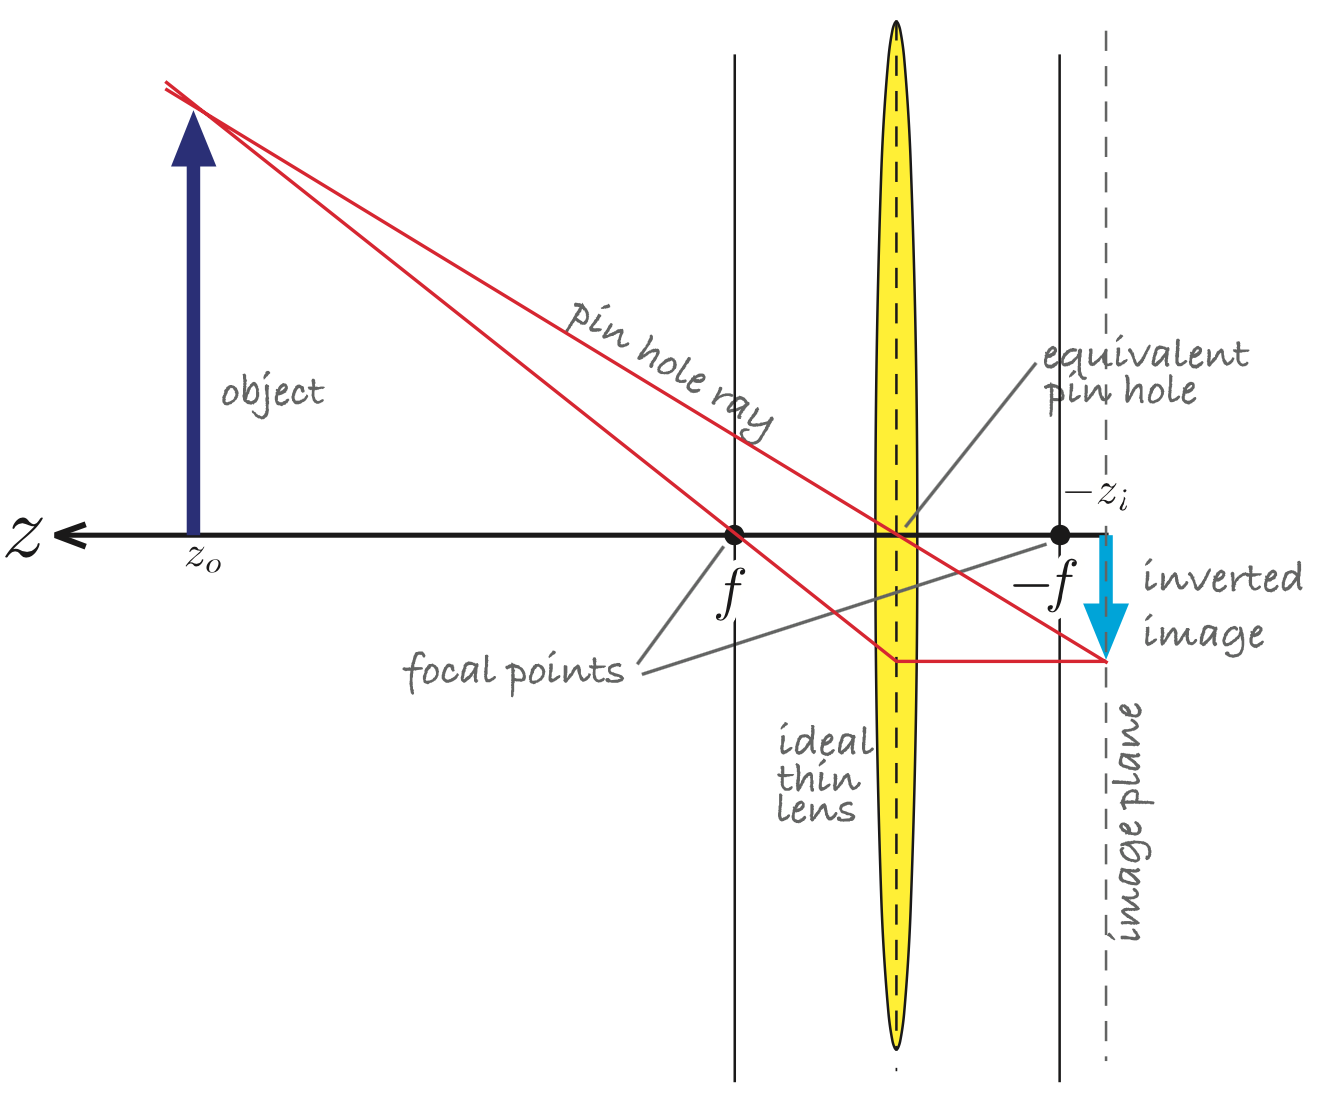
\includegraphics[width=.7\textwidth]{thinLensModel}
\end{figure}
\begin{itemize}
\item More light, but images are not always in focus.
\item 
\end{itemize}
\end{frame}

\begin{frame}
\frametitle{Thin lens model}
\begin{figure}[!h]
\centering
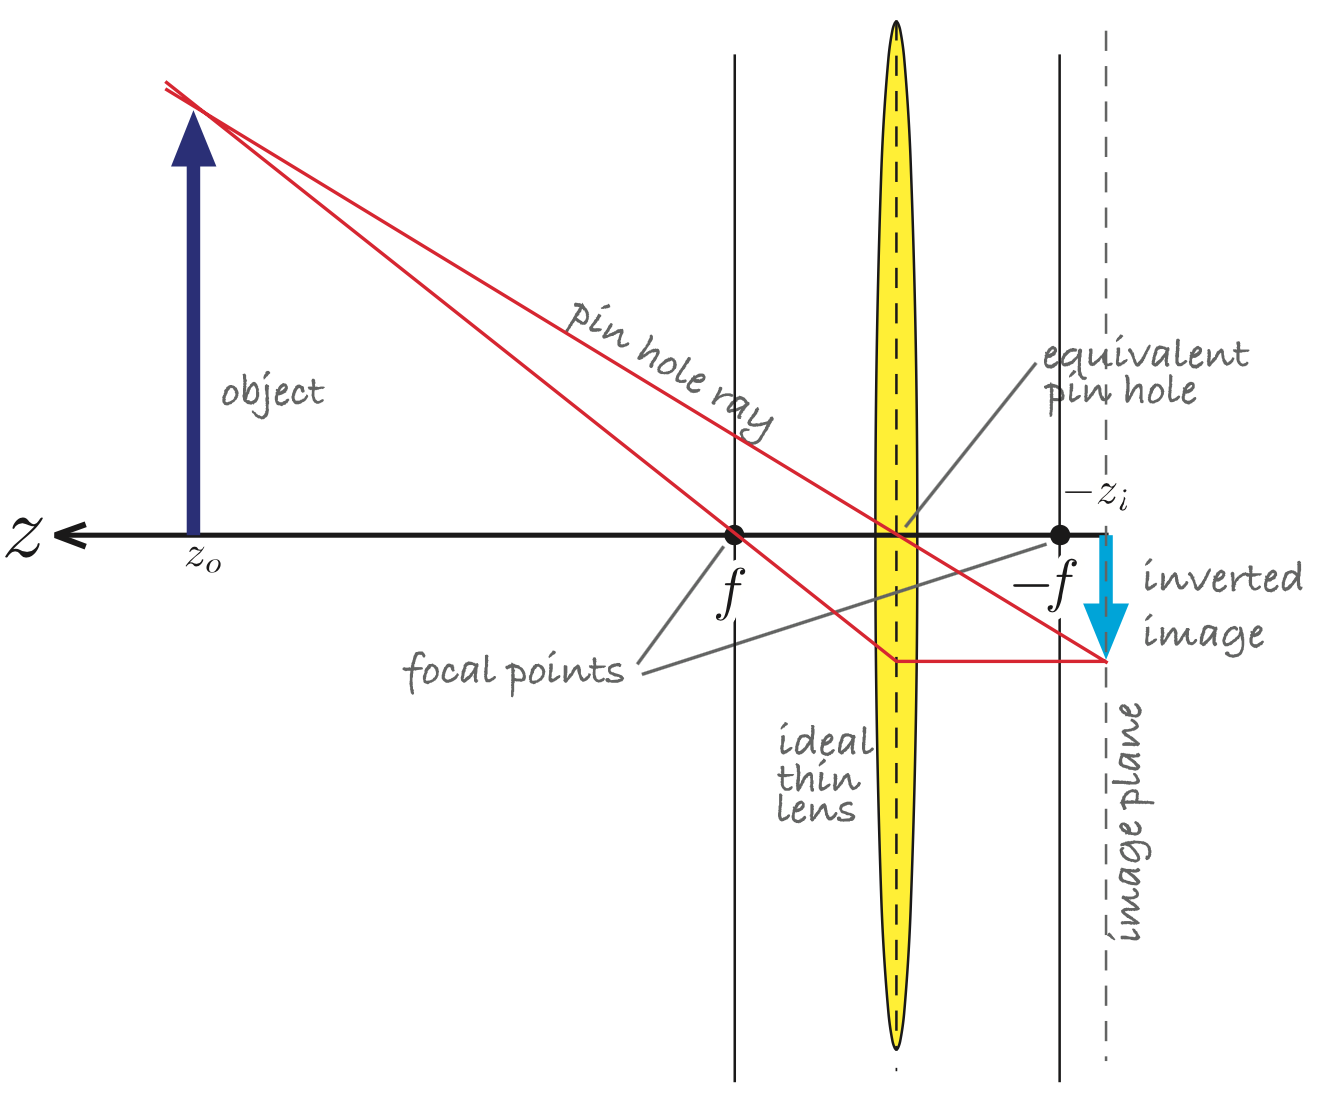
\includegraphics[width=.3\textwidth]{thinLensModel}
\end{figure}
\begin{itemize}
\item Thin-lens equation
\[
\dfrac{1}{z_0} + \dfrac{1}{z_{i}} = \dfrac{1}{f}
\]
\item If $z_o \mapsto \infty$ then $z_i \mapsto f$.
\end{itemize}
\end{frame}

\section{Perspective Projection}

\begin{frame}
\begin{columns}
\begin{column}{.6\textwidth}
\begin{figure}[!h]
\centering
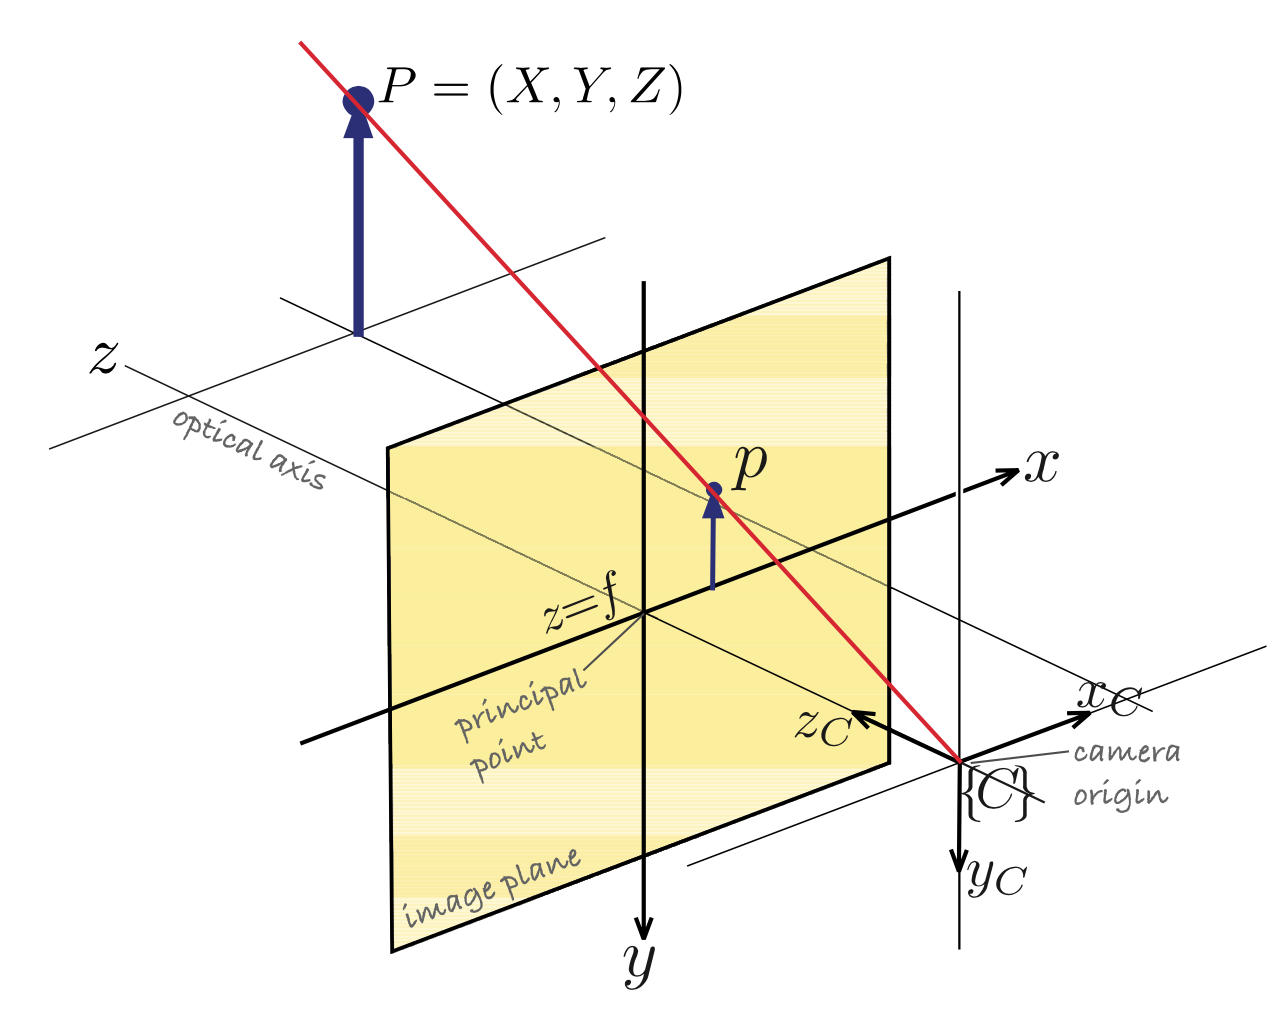
\includegraphics[width=\textwidth]{perspectiveProjModel}
\end{figure}
\end{column}
\begin{column}{.5\textwidth}
Perspective projection:
\begin{itemize}
\item $x = \dfrac{fX}{Z}$.
\item $y = \dfrac{fY}{Z}$.
\item 3D to 2D.
\item $\mathbb{R}^{3} \mapsto \mathbb{R}^{2}$.
\item One dimension lost.
\end{itemize}
\end{column}
\end{columns}
\end{frame}

\begin{frame}
\begin{figure}[!h]
\centering
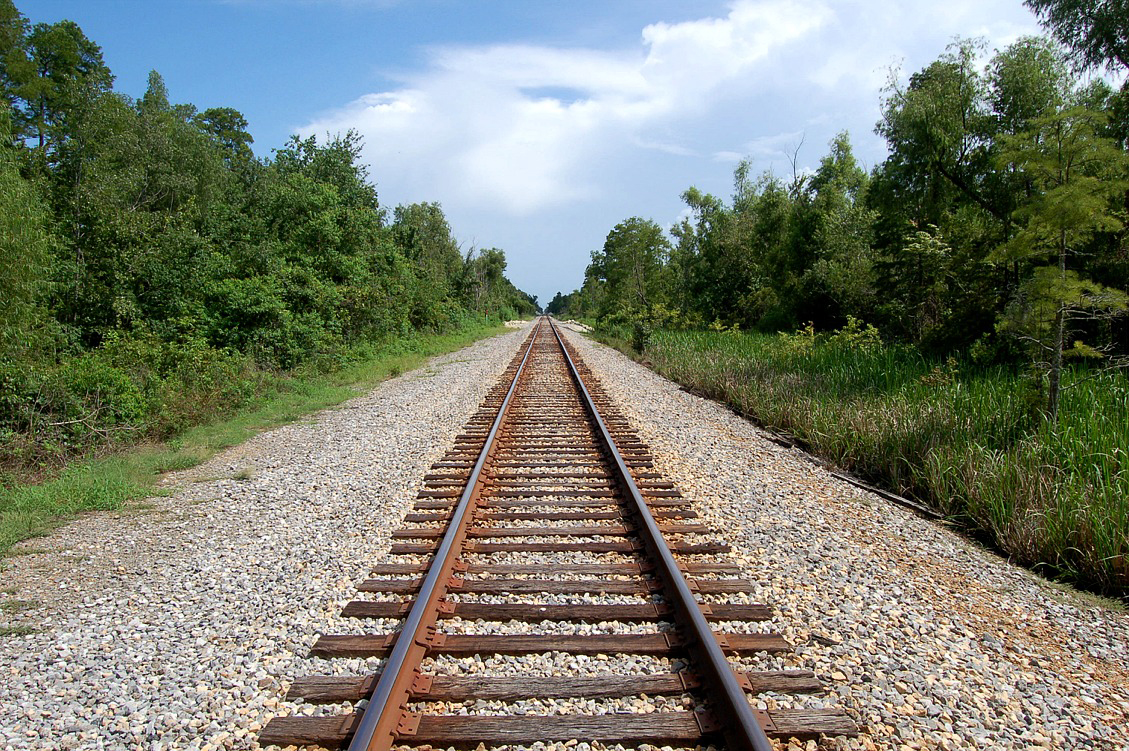
\includegraphics[width=\textwidth]{railroad}
\end{figure}
\end{frame}

\begin{frame}
\begin{figure}[!h]
\centering
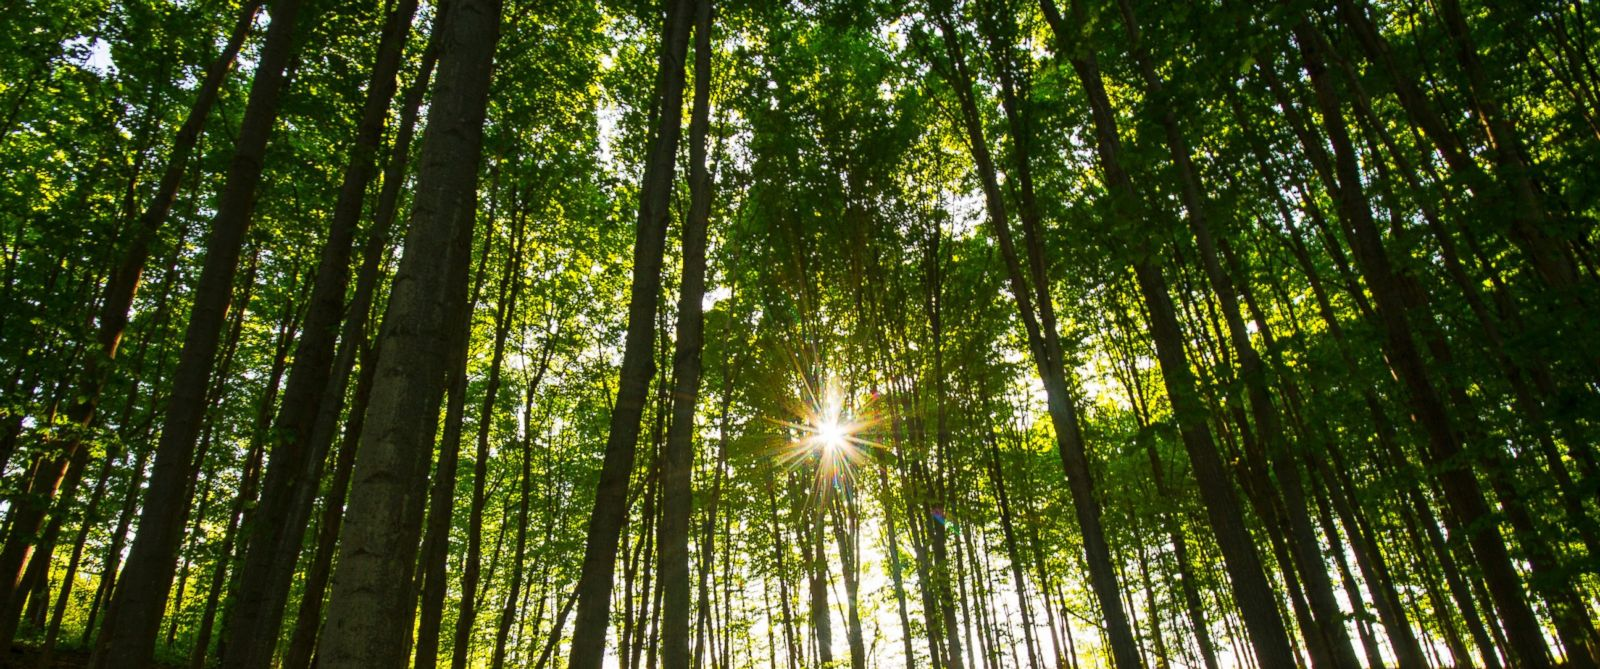
\includegraphics[width=\textwidth]{trees}
\end{figure}
\end{frame}

\begin{frame}
\begin{figure}[!h]
\centering
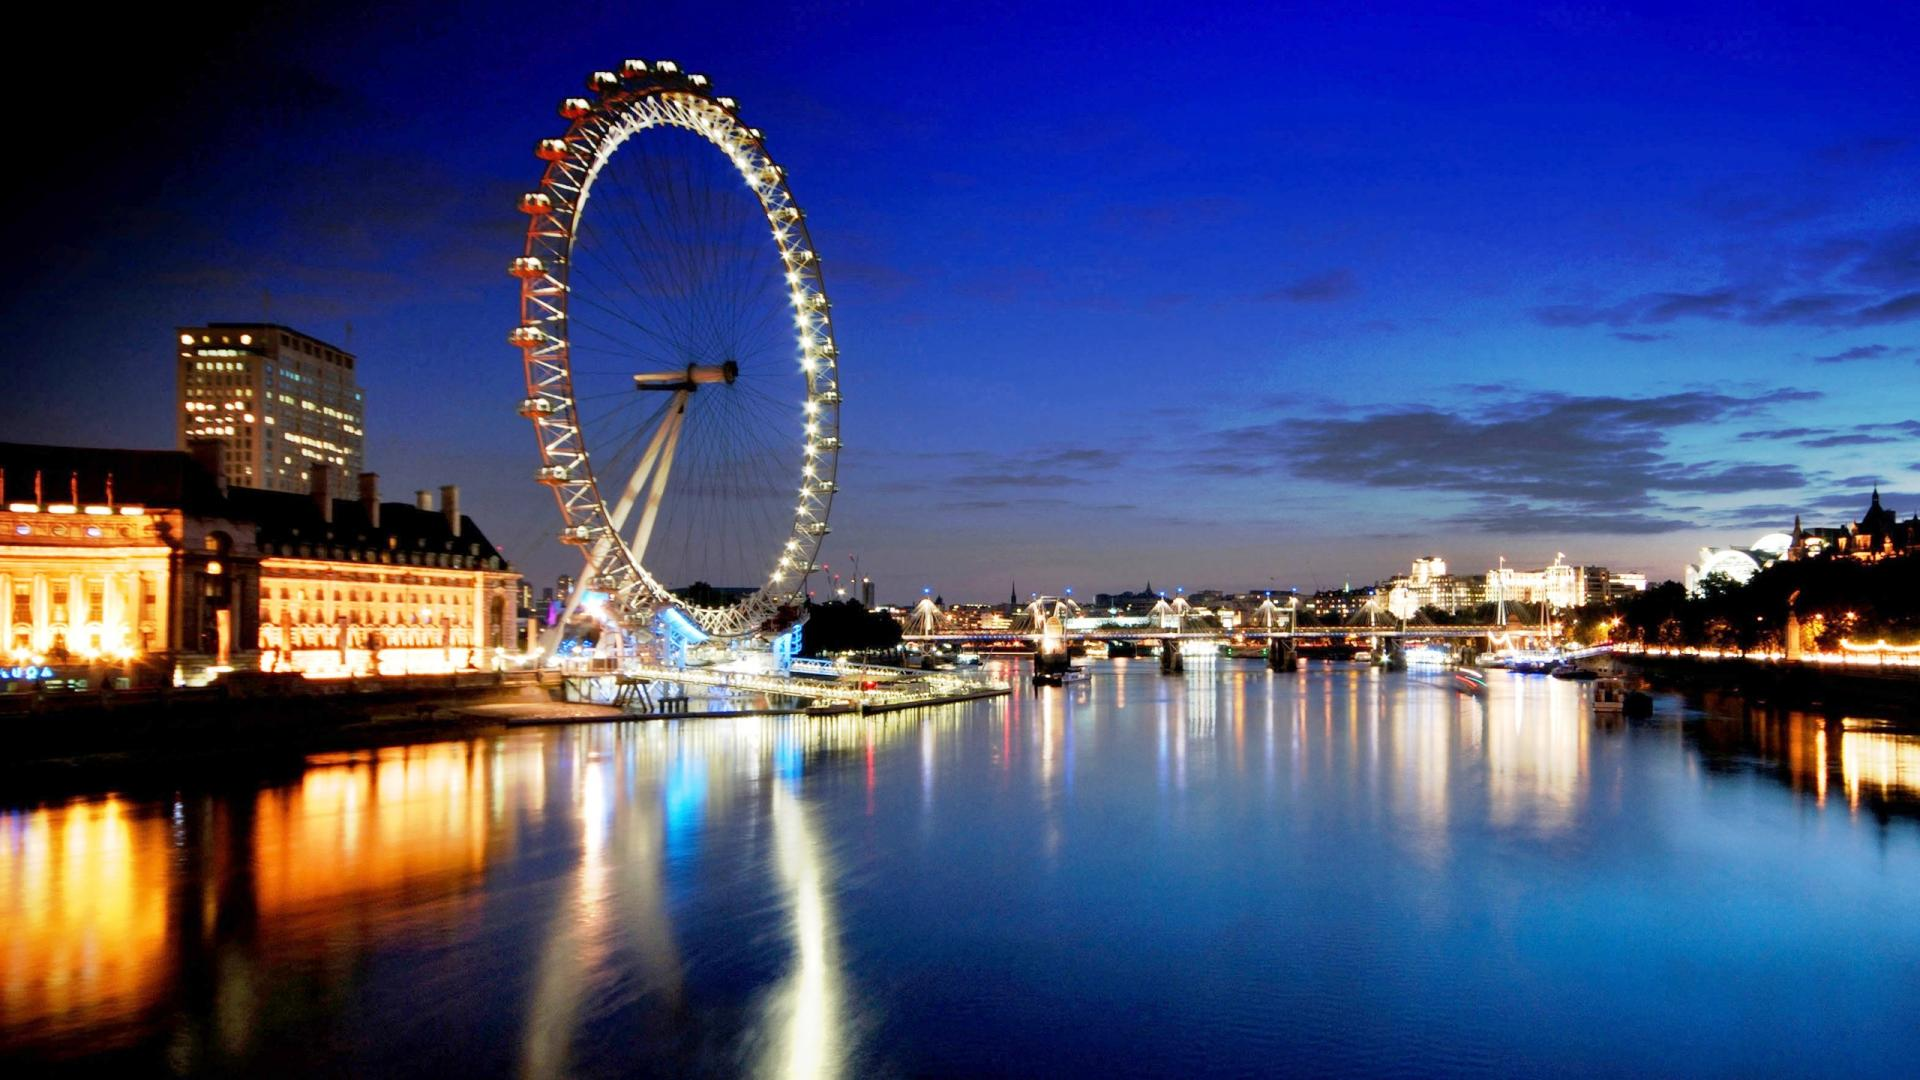
\includegraphics[width=\textwidth]{ferriswheel}
\end{figure}
\end{frame}

\begin{frame}
\frametitle{Perspective Projection}
\begin{itemize}
\item Lines $\mapsto$ lines
\begin{itemize}
\item Parallel lines no necessarily parallel.
\item Angles are not preserved.
\end{itemize}
\item Conics $\mapsto$ conics.
\end{itemize}
\begin{figure}[!h]
\centering
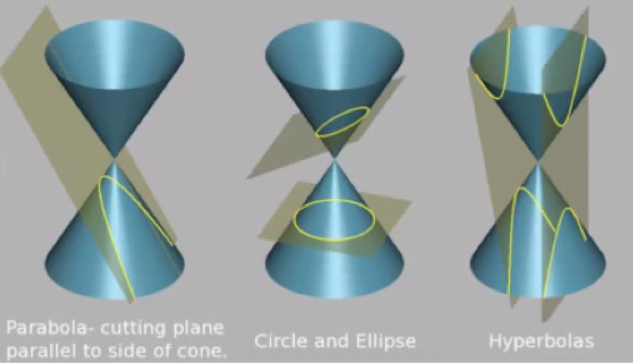
\includegraphics[width=.5\textwidth]{conics}
\end{figure}
\end{frame}

\begin{frame}
\begin{figure}[!h]
\centering
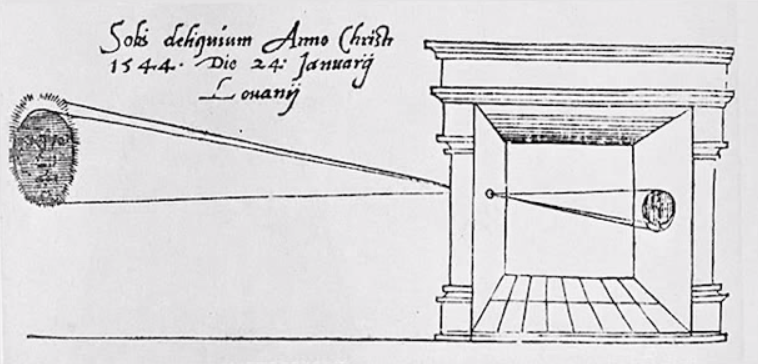
\includegraphics[width=.8\textwidth]{scaling}
\end{figure}
\end{frame}

\begin{frame}
\begin{figure}[!h]
\centering
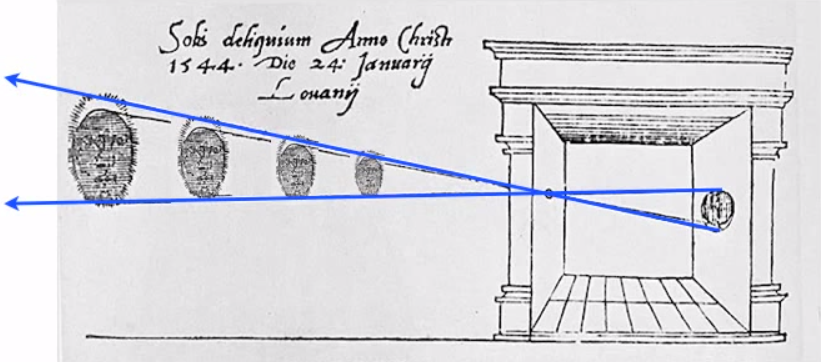
\includegraphics[width=.8\textwidth]{scaling2}
\end{figure}
\end{frame}

\section{Homogeneous Coordinates}

\begin{frame}
\frametitle{Homogeneous coordinates}
\begin{columns}
\begin{column}{.5\textwidth}
\begin{itemize}
\item Cartesian $\mapsto$ Homogeneous:
\end{itemize}
\[
\begin{array}{cc}
\textbf{P} = \left ( x, y \right ) & \tilde{\textbf{P}} = \left ( x, y, 1 \right ) \\
\textbf{P} \in \mathbb{R}^2 & \tilde{\textbf{P}} \in \mathbb{P}^2
\end{array}
\]
\begin{itemize}
\item Homogeneous $\mapsto$ Cartesian:
\end{itemize}
\[
\begin{array}{cc}
\tilde{\textbf{P}} = \left ( \tilde{x}, \tilde{y}, \tilde{z} \right ) \mapsto \textbf{P} = \left ( x, y \right )
\end{array}
\]
where
\[
x = \tilde{x}/\tilde{z},\ \ y = \tilde{y}/\tilde{z}.
\]
\end{column}
\begin{column}{.5\textwidth}
\begin{figure}[!h]
\centering
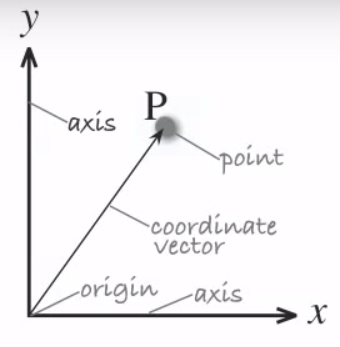
\includegraphics[width=\textwidth]{axes}
\end{figure}
\end{column}
\end{columns}
\end{frame}

\section{Central Projection Model}

\begin{frame}
\frametitle{Central Projection Model}
\[
\left (
\begin{array}{c}
\tilde{x}\\
\tilde{y}\\
\tilde{z}
\end{array}
\right )
=
\left (
\begin{array}{cccc}
f & 0 & 0 & 0 \\
0 & f & 0 & 0 \\
0 & 0 & 1 & 0
\end{array}
\right )
\left (
\begin{array}{c}
X \\
Y \\
Z \\
1
\end{array}
\right )
\]
I.e.,
\[
\tilde{x} = fX,\ \ \tilde{y} = fY,\ \ \tilde{z} = Z.
\]
As before:
\[
x = \tilde{x}/\tilde{z},\ \ y = \tilde{y}/\tilde{z}.
\]
\[
\mapsto x = \dfrac{fX}{Z},\ \ y = \dfrac{fY}{Z}
\]
\begin{itemize}
\item Perspective transformation, with the divide by $Z$ is \textbf{linear} in homogeneous coordinate form.
\end{itemize}
\end{frame}

\begin{frame}
\frametitle{Central Projection Model}
\[
\left (
\begin{array}{c}
\tilde{x}\\
\tilde{y}\\
\tilde{z}
\end{array}
\right )
=
\left (
\begin{array}{cccc}
f & 0 & 0 & 0 \\
0 & f & 0 & 0 \\
0 & 0 & 1 & 0
\end{array}
\right )
\left (
\begin{array}{c}
X \\
Y \\
Z \\
1
\end{array}
\right )
\]
%
\[
\left (
\begin{array}{c}
\tilde{x}\\
\tilde{y}\\
\tilde{z}
\end{array}
\right )
=
\underbrace{
\left (
\begin{array}{cccc}
1 & 0 & 0 & 0 \\
0 & 1 & 0 & 0 \\
0 & 0 & 1 & 0
\end{array}
\right )
}_{3D \mapsto 2D}
\underbrace{
\left (
\begin{array}{cccc}
f & 0 & 0 & 0 \\
0 & f & 0 & 0 \\
0 & 0 & 1 & 0 \\
0 & 0 & 0 & 1
\end{array}
\right )
}_{\text{scaling/zooming}}
\left (
\begin{array}{c}
X \\
Y \\
Z \\
1
\end{array}
\right )
\]
\end{frame}

\begin{frame}
\begin{figure}[!h]
\centering
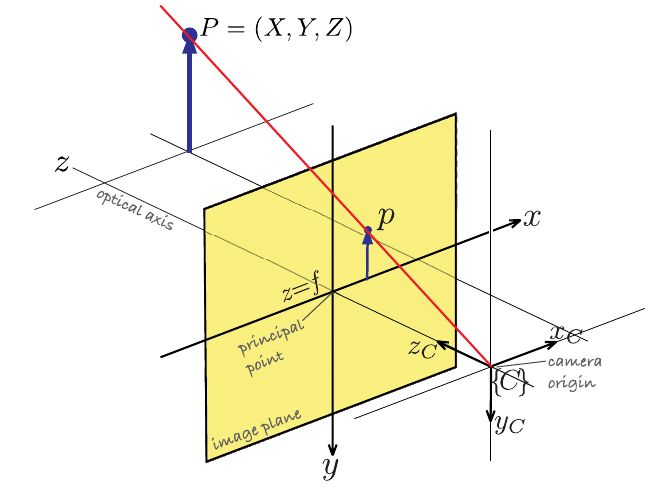
\includegraphics[width=.5\textwidth]{centralProjModel}
\end{figure}
\[
\left (
\begin{array}{c}
\tilde{x}\\
\tilde{y}\\
\tilde{z}
\end{array}
\right )
=
\left (
\begin{array}{cccc}
f & 0 & 0 & 0 \\
0 & f & 0 & 0 \\
0 & 0 & 1 & 0
\end{array}
\right )
\left (
\begin{array}{c}
X \\
Y \\
Z \\
1
\end{array}
\right )
\]
\end{frame}

\begin{frame}
\begin{figure}[!h]
\centering
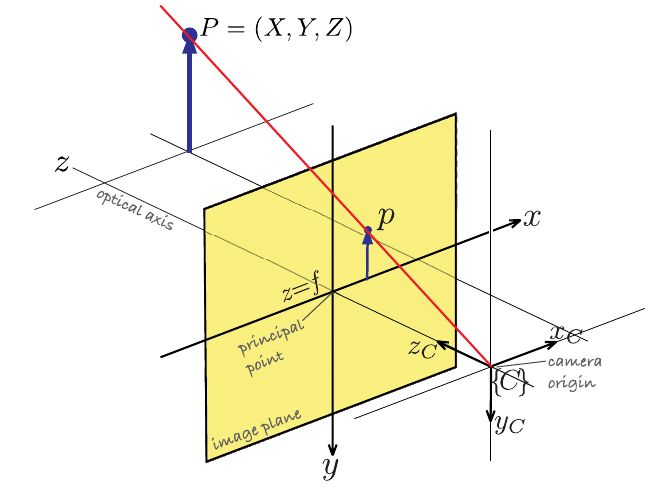
\includegraphics[width=.5\textwidth]{centralProjModel}
\end{figure}
\[
\left (
\begin{array}{ccc}
\dfrac{1}{\rho_u} & 0 & u_{0} \\
0 & \dfrac{1}{\rho_v} & v_{0} \\
0 & 0 & 1
\end{array}
\right )
\]
\end{frame}

\begin{frame}
\begin{columns}
\begin{column}{.5\textwidth}
\begin{figure}[!h]
\centering
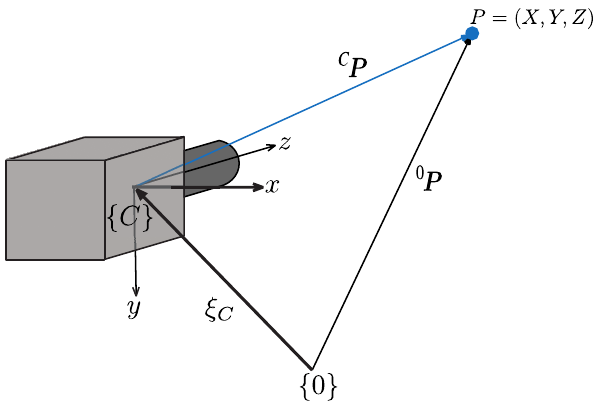
\includegraphics[width=\textwidth]{camera}
\end{figure}
\end{column}
\begin{column}{.5\textwidth}
\[
\left (
\begin{array}{c}
\tilde{x}\\
\tilde{y}\\
\tilde{z}
\end{array}
\right )
=
\left (
\begin{array}{cccc}
f & 0 & 0 & 0 \\
0 & f & 0 & 0 \\
0 & 0 & 1 & 0
\end{array}
\right )
\left (
\begin{array}{c}
X \\
Y \\
Z \\
1
\end{array}
\right )
\]
\end{column}
\end{columns}
\[
\left (
\begin{array}{c}
\tilde{u} \\
\tilde{v} \\
\tilde{w}
\end{array}
\right )
=
\left (
\begin{array}{ccc}
\dfrac{1}{\rho_u} & 0 & u_{0} \\
0 & \dfrac{1}{\rho_v} & v_{0} \\
0 & 0 & 1
\end{array}
\right )
\left (
\begin{array}{cccc}
f & 0 & 0 & 0 \\
0 & f & 0 & 0 \\
0 & 0 & 1 & 0
\end{array}
\right )
\left (
\begin{array}{cc}
\textbf{\text{R}} & t \\
\textbf{\text{0}}_{1\times 3} & 1
\end{array}
\right )^{-1}
\left (
\begin{array}{c}
X \\
Y \\
Z \\
1
\end{array}
\right )
\]
\end{frame}

\begin{frame}
\begin{figure}[!h]
\centering
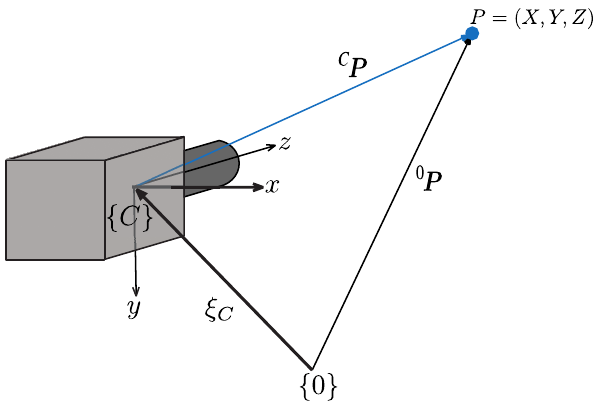
\includegraphics[width=.5\textwidth]{camera}
\end{figure}
\[
\left (
\begin{array}{c}
\tilde{u} \\
\tilde{v} \\
\tilde{w}
\end{array}
\right )
=
\underbrace{
\left (
\begin{array}{ccc}
\dfrac{1}{\rho_u} & 0 & u_{0} \\
0 & \dfrac{1}{\rho_v} & v_{0} \\
0 & 0 & 1
\end{array}
\right )
\left (
\begin{array}{cccc}
f & 0 & 0 & 0 \\
0 & f & 0 & 0 \\
0 & 0 & 1 & 0
\end{array}
\right )
}_{\text{Intrinsic parameters}}
\underbrace{
\left (
\begin{array}{cc}
\textbf{\text{R}} & t \\
\textbf{\text{0}}_{1\times 3} & 1
\end{array}
\right )^{-1}
}_{\text{Extrinsic parameters}}
\left (
\begin{array}{c}
X \\
Y \\
Z \\
1
\end{array}
\right )
\]
\end{frame}

\begin{frame}
\begin{figure}[h]
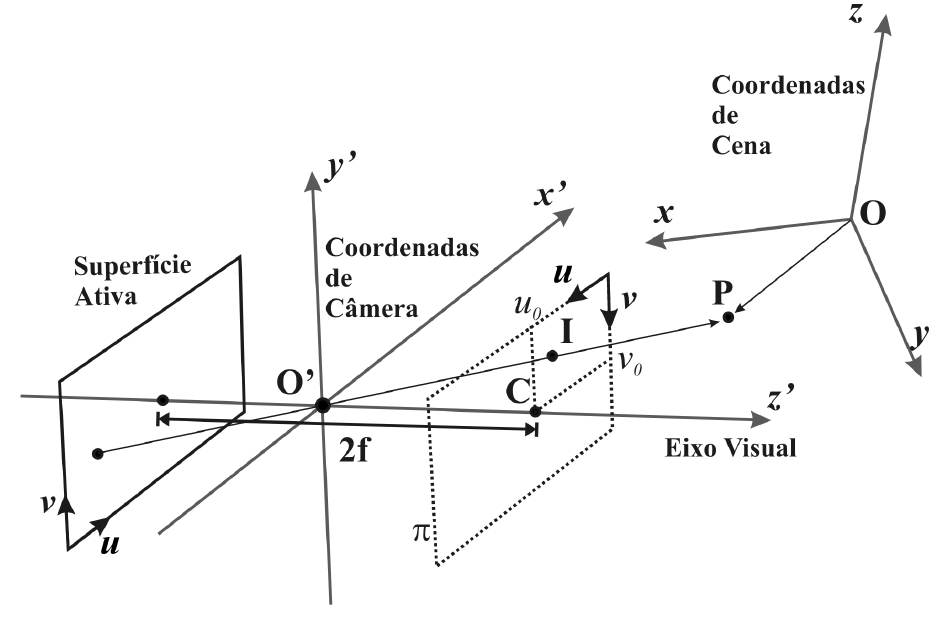
\includegraphics[width=\textwidth]{coord}
\end{figure}
\end{frame}

\begin{frame}
\begin{columns}
\begin{column}{.5\textwidth}
\begin{figure}[!h]
\centering
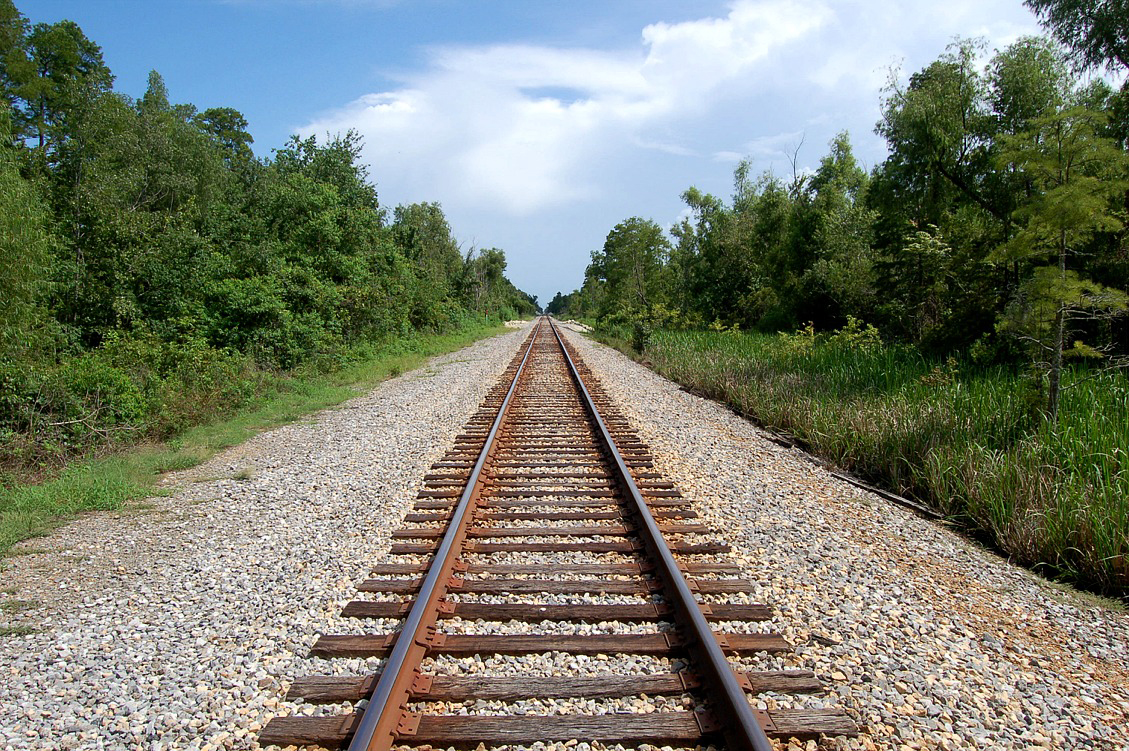
\includegraphics[width=\textwidth]{railroad}
\end{figure}
\end{column}
\begin{column}{.5\textwidth}
\begin{figure}[!h]
\centering
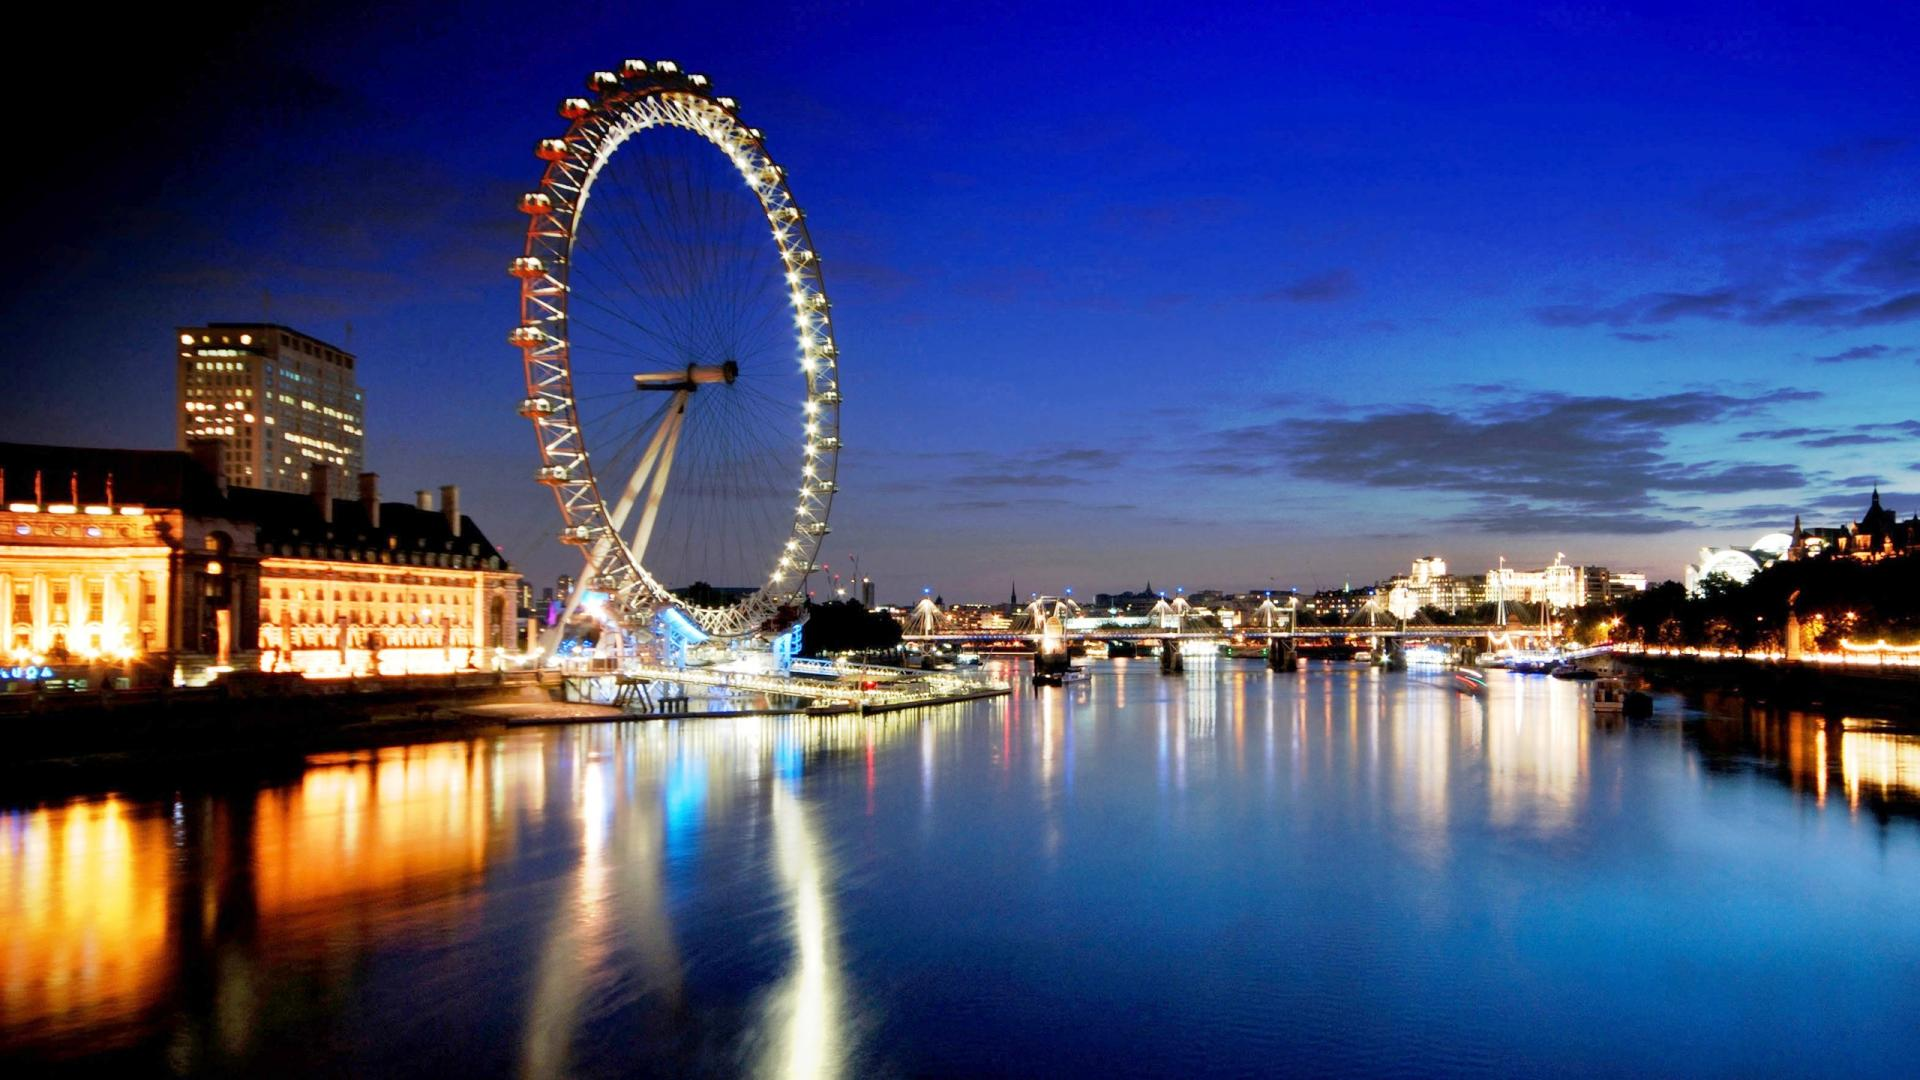
\includegraphics[width=\textwidth]{ferriswheel}
\end{figure}
\end{column}
\end{columns}
\end{frame}

\begin{frame}
\begin{figure}[!h]
\centering
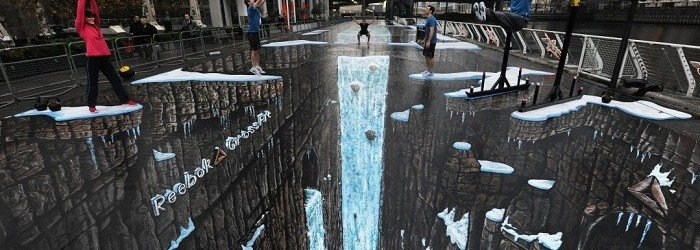
\includegraphics[width=\textwidth]{illusion}
\end{figure}
\end{frame}

\section{Other camera types}

\begin{frame}
\frametitle{Fish-eye lens}
\begin{columns}
\begin{column}{.5\textwidth}
\begin{figure}[!h]
\centering
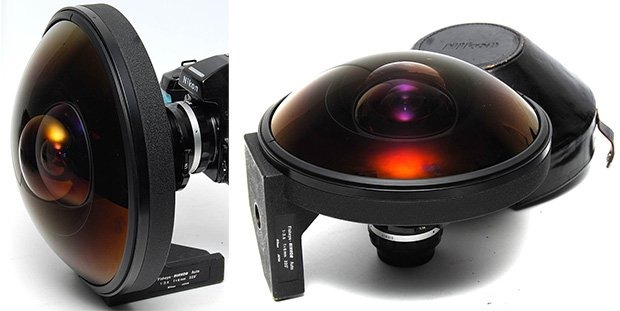
\includegraphics[width=\textwidth]{nikonfisheye}
\end{figure}
\end{column}
\begin{column}{.5\textwidth}
\begin{figure}[!h]
\centering

\includegraphics[width=.5\textwidth]{fisheyemugshot}
\end{figure}
\begin{figure}[!h]
\centering
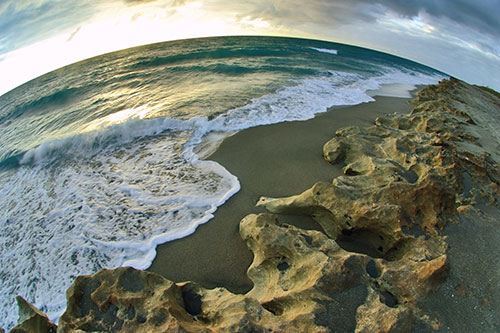
\includegraphics[width=\textwidth]{fisheyehorizon}
\end{figure}
\end{column}
\end{columns}
\end{frame}

\begin{frame}
\frametitle{Imaging by reflection}
\begin{columns}
\begin{column}{.5\textwidth}
\begin{figure}[!h]
\centering
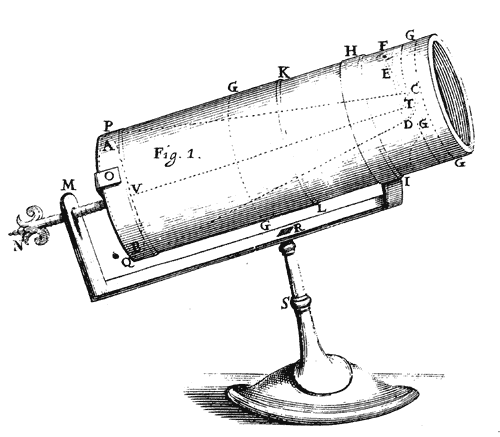
\includegraphics[width=.7\textwidth]{telescope}
\caption{An accompt of a new catadioptrical telescope invented by Mr. Isaac Newton ($\approx$1670)}
\end{figure}
\end{column}
\begin{column}{.5\textwidth}
\begin{figure}[!h]
\centering
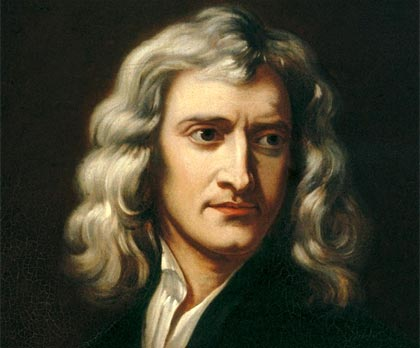
\includegraphics[width=.4\textwidth]{newton}
\end{figure}
\begin{figure}[!h]
\centering
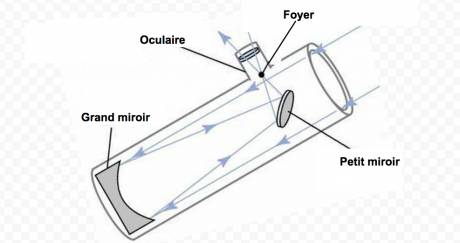
\includegraphics[width=\textwidth]{newton-telescope}
\end{figure}
\end{column}
\end{columns}
\end{frame}

\begin{frame}
\frametitle{Spherical reflection}
\begin{figure}[!h]
\centering
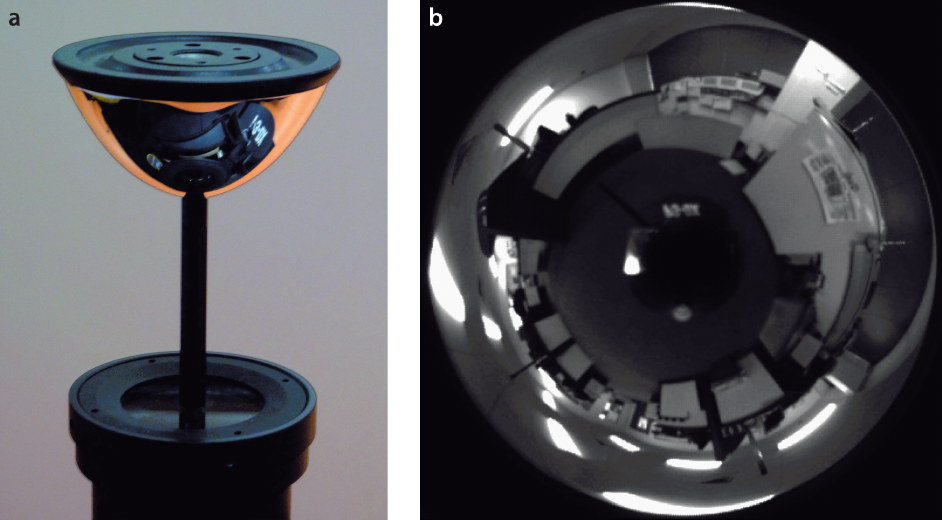
\includegraphics[width=.7\textwidth]{catadioptric}
\end{figure}
\end{frame}

\begin{frame}
\begin{figure}[!h]
\centering
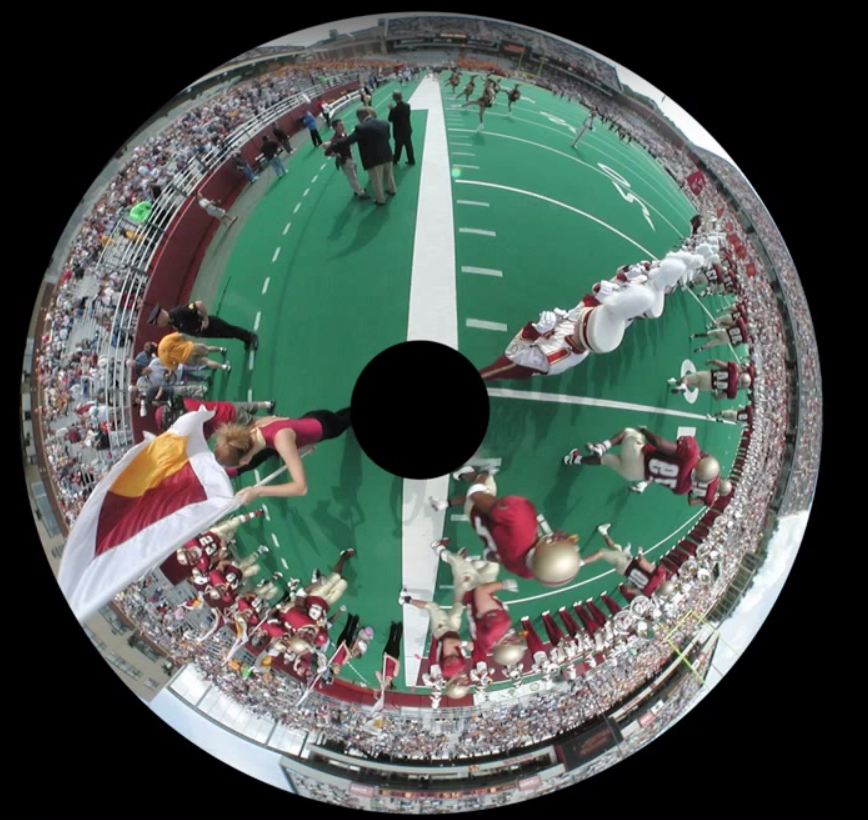
\includegraphics[width=.7\textwidth]{parade}
\end{figure}
\end{frame}

\section{Light field}

\begin{frame}
\frametitle{Light field}
\begin{itemize}
\item A function that describes the amount of light travelling in \textbf{every direction} at \textbf{every point} in space.
\item A light field sensor captures the color, intensity and vector \textbf{direction} of the rays of light.
\begin{itemize}
\item a traditional camera simply adds up all the light rays and record a single amount of light
\end{itemize}
\item Given the lightfield we can compute the image from any position.
\end{itemize}
\end{frame}

\begin{frame}
\begin{figure}[!h]
\centering
\includegraphics[width=\textwidth]{matrix}
\end{figure}
\end{frame}

\begin{frame}
\begin{figure}[!h]
\centering
\includegraphics[width=\textwidth]{focusProblem}
\end{figure}
\end{frame}

\begin{frame}
\begin{figure}[!h]
\centering
\includegraphics[width=\textwidth]{focusProblem2}
\end{figure}
\end{frame}

\begin{frame}
\begin{columns}
\begin{column}{.5\textwidth}
\begin{figure}[!h]
\centering
\includegraphics[width=.9\textwidth]{lightfieldcam3}
\end{figure}
\end{column}
\begin{column}{.5\textwidth}
\begin{figure}[!h]
\centering
\includegraphics[width=.9\textwidth]{lytro_light_field_camera_1}
\end{figure}
\end{column}
\end{columns}
\begin{itemize}
\item \url{https://www.lytro.com/}
\item \url{http://www.diyphotography.net/how-light-field-photography-works/}
\item \url{https://vimeo.com/130983212}
\end{itemize}
\end{frame}

%\section{References}
%
%\begin{frame}
%\frametitle{References}
%\begin{enumerate}
%\item Cork, P., ``\textit{Robotics, Vision and Control.}''. Springer, 2011.
%\end{enumerate}
%\end{frame}

\begin{frame}
\frametitle[alignment=center]{}
\flushbottom
\centering
Thank you!\\
\href{mailto:tiago@ic.ufal.br}{tvieira@ic.ufal.br}\\
%\href{mailto:warley.barbosa@edge.ufal.br}{warley.barbosa@edge.ufal.br}\\
%\href{mailto:icaro.bastos@edge.ufal.br}{icaro.bastos@edge.ufal.br}\\
\end{frame}


\end{document}